\documentclass[a4paper,12pt]{book}
\usepackage[utf8]{inputenc}
\usepackage[a-1b]{pdfx} % to generate valid PDFA
                 % see https://www.mathstat.dal.ca/~selinger/pdfa/ for details
\usepackage{graphicx}
\graphicspath{ {images/} }
\usepackage{caption}
\usepackage{subcaption}
\usepackage{sublabel}
\usepackage{hyperref}
\hypersetup{hidelinks}
\usepackage[english]{babel}
\usepackage{blindtext}
\usepackage{amsfonts} 
\usepackage{amsmath}
\usepackage{mathtools}
\usepackage{bbold}
\usepackage{derivative}
\usepackage{bm}
\usepackage{enumitem}  
\usepackage[a4paper,width=150mm,top=25mm,bottom=25mm,bindingoffset=6mm]{geometry}
\usepackage{setspace} \onehalfspacing 

% page size tuning:
%\setlength{\oddsidemargin}{8mm}   % Distance from the left edge -1 inch
%\setlength{\textwidth}{145mm}     % Horizontal width of the standard text
%\setlength{\topmargin}{2mm}       % Distance from top to PAGE'S HEAD -1 inch
%\setlength{\textheight}{225mm}    % Vertical length of the page body
%\setlength{\headheight}{0mm}      % Height of a box containing the head
%\setlength{\parskip}{0.5mm}       % Extra vertical space before a paragraph
%\setlength{\parindent}{9mm}       % Indentation at paragraph beginning
%\linespread{1.12}                 % Line-to-line spacing
%\renewcommand{\floatpagefraction}{.93} % for text coexisting with figs and tabs
%\renewcommand{\textfraction}{0.02}% more or less equiv. to the above

\usepackage[backend=biber,style=ext-numeric-comp,sorting=none,isbn=false, issn=false, doi=false, url=false, number=false ,date=year,dashed=false,  naturbib]{biblatex}
\newbibmacro{string+doi}[1]{%
  \iffieldundef{doi}{#1}{\href{http://dx.doi.org/\thefield{doi}}{#1}}}
\DeclareFieldFormat{title}{\usebibmacro{string+doi}{\mkbibemph{#1}}}
\DeclareFieldFormat[article]{title}{\usebibmacro{string+doi}{\mkbibquote{#1}}}
\DeclareFieldFormat[article,periodical]{volume}{\mkbibbold{#1}}
\DeclareFieldFormat{journaltitle}{#1\isdot}
\addbibresource{references.bib}

\newcommand{\Autoref}[1]{%
  \begingroup%
  \def\chapterautorefname{Chapter}%
  \def\sectionautorefname{Section}%
  \def\subsectionautorefname{Subsection}%
  \autoref{#1}%
  \endgroup%
}

% Use \usepackage[warnundef]{jabbrv} to show undefined abbreviation warnings
\usepackage{jabbrv}
% Old-school compressed citations:
%\usepackage{cite}
% New way for compressed citations (hyperref compatible):
%\usepackage[numbers,sort&compress]{natbib}


\usepackage[acronym]{glossaries}
\makeglossaries
\newacronym{fpe}{\textsc{fpe}}{Fokker-Planck Equation}
\newacronym{fpo}{\textsc{fpo}}{Fokker-Planck Operator}
\newacronym{pmf}{\textsc{pmf}}{Probability Mass Function}
\newacronym{pdf}{\textsc{pdf}}{Probability Density Function}
\newacronym{ndf}{\textsc{ndf}}{Number Density Function}
\newacronym{lhc}{\textsc{lhc}}{Large Hadron Collider}
\newacronym{ode}{\textsc{ode}}{Ordinary Differential Equation}
\newacronym{pde}{\textsc{pde}}{Partial Differential Equation}
\newacronym{sde}{\textsc{sde}}{Stochastic Differential Equation}
\newacronym{fdr}{\textsc{fdr}}{Fluctuation-Dissipation Relation}
\newacronym{qgp}{\textsc{qgp}}{Quark-Gluon Plasma}
\newacronym{com}{\textsc{com}}{Center-of-Momentum Frame}
\newacronym{qcd}{\textsc{qcd}}{Quantum Chromodynamics}
\newacronym{dis}{\textsc{dis}}{Deep Inelastic Scattering}
\newacronym{cgc}{\textsc{cgc}}{Color-Glass Condensate}


\begin{document}


\begin{titlepage}
    \begin{center}
        \vspace*{1cm}
            
        \Huge
        \textbf{Algebraic methods of solution of a Fokker-Planck equation in heavy-ions collisions}
            
        \vspace{0.5cm}
        \LARGE
        Thesis Subtitle
            
        \vspace{1.5cm}
            
        \textbf{Alessandro Rizzi}
            
        \vfill
            
        A thesis presented for the degree of\\
        M.s.C. Physics
            
        \vspace{0.8cm}

        \Large
        \textit{Referees:}\\
        Prof. Georg Wolschin
            
        \vspace{0.8cm}    
        \Large
        Department of Physics and Astronomy\\
        Heidelberg University\\
        Germany\\
        December 2023
            
    \end{center}
\end{titlepage}

\thispagestyle{plain}

\begin{center}
    \vspace{0.9cm}
    \textbf{Zusammenfassung}
\end{center}
\blindtext

\begin{center}
    \vspace{0.9cm}
    \textbf{Abstract}
\end{center}


The aim of this thesis is to describe baryon stopping and charged hadron thermalization in heavy-ion collisions by means of a non-equilibrium statistical model. The particle's phase-space trajectories are treated as a drift-diffusion stochastic process, leading to a Fokker-Planck equation (\acrshort{fpe}) for the single-particle probability distribution function.
The drift and diffusion coefficients are derived from the expected asymptotic state via appropriate fluctuation-dissipation relations, and the resulting non-linear \acrshort{fpe} is then numerically solved with a spectral eigenfunction decomposition. The obtained time-dependent particle distribution is then compared to experimental data from the Large Hadron Collider (\acrshort{lhc}), to tune the free parameters of the model. 



\tableofcontents
\printglossary[type=\acronymtype]


\chapter{Introduction}

In~\autoref{chap:stochastic}, I introduce the concepts of random variables and (relativistic) stochastic calculus, focusing on the Fokker-Planck formulation of drift-diffusion processes. 

\Autoref{chap:heavy-ions} contains an introduction to spectral methods of solution of partial differential equations and develops the spectral formulation of the \acrshort{fpe} used in this thesis.

In~\autoref{chap:particle_therm}, I outline the physical process and its formulation in the stochastic drift-diffusion process framework introduced in~\autoref{chap:stochastic}.
The model's results are then presented and compared to experimental data from LHC.

Finally,~\autoref{chap:conclusions} discuss the obtained results, the advantages and limits of the employed approach to heavy-ions collisions and possible future improvements.


\chapter{Probability theory and stochastic processes}\label{chap:stochastic}
In the realm of physics, a profound understanding of uncertainty and random behavior is essential for describing and predicting natural phenomena. Probability theory and stochastic processes provide the mathematical framework to tackle these challenges. %chatgpt
Standard textbooks are~\textcite{gardiner2009stochastic} and~\textcite{pavliotis2014stochastic}, as the report by~\textcite{HANGGI1982207}. A short and practical course can be found in~\textcite{Schwarz19} lecture notes.

\section{Basis of probability theory}

Before studying a stochastic process, we have to briefly introduce the mathematical framework of probability theory. Following the rigorous axiomatic approach introduced by~\textcite{kolmogorov1933}, we start by considering the set of all possible outcomes of a measure, the \textit{sample space} $\Omega$, that we ask to be \textit{measurable}. We define an \textit{event} $A \subseteq \Omega$ as a subset of the sample space and $\omega \in \Omega$ as a single outcome of the experiment. $\emptyset$ is the \textit{empty set}, that contains no events.

Using the most classical of examples, if our experiment is throwing an ordinary six-faced dice, the sample space $\Omega$ would be getting any number from one to six, an event $A$ getting e.g. an odd number, and $\omega$ getting a specific number. In the context of this thesis, $\Omega$ will be the continuous phase space of a relativistic particle measured by a detector at the end of a complex interaction that we model with a stochastic process. \\

To assign probabilities to events, we introduce the \textit{$\sigma$-algebra} $\mathcal{F}$. This is a collection of subsets of $\Omega$ that contains the entire sample space and is closed under complementation and countable unions. $\mathcal{F}$ serves a crucial role in defining the concept of probability, as it restricts which events or sets of outcomes can be assigned probabilities within the sample space $\Omega$. For example, when $\Omega$ is uncountable, not all subsets of the sample space need to be events. 

As a relevant physical example, let $\Omega = \mathbb{R}^n $. The $\sigma$-algebra generated by the open subset (open balls) of $\mathbb{R}^n$ is called the \textit{Borel $\sigma$-algebra}, denoted by  $\mathcal{B}(\mathbb{R}^n)$. If $G$ is a closed subset of $\mathbb{R}^n$, we can define analogously its Borel $\sigma$-algebra $\mathcal{B}(G)$.\\


A \textit{probability measure} $P$ is a function that assigns a real number in the interval $[0, 1]$ to each event in the $\sigma$-algebra $\mathcal{F}$, satisfying the following \textit{probability axioms}: 
\begin{enumerate}[label=\roman*)]
    \item $P(A) \geq 0$ for all $A \in \mathcal{F}$ 
    \item $P(\Omega)=1$
    \item If $A_i(i=1,2,3 \ldots)$ is a countable collection of non-overlapping sets, $A_i \cap A_j=\emptyset$ for all $i \neq j$, then
$$
P\left(\bigcup_i A_i\right)=\sum_i P\left(A_i\right)
$$
\end{enumerate}

From these three fundamental axioms, it follows:

\begin{enumerate}[label=\roman*)]
  \setcounter{enumi}{3}
    \item  if $\bar{A}$ is the complement of $A$, i.e., the set of all events not contained in $A$, then
$$
P(\bar{A})=1-P(A),
$$
    \item $P(\emptyset)=0$
    %\item $P(A) \leq 1 \; \forall A$
\end{enumerate}

The axiomatic construction of probability, while providing a solid formal mathematical framework, requires that the \textit{probability space} $(\Omega,\mathcal{F}, P)$ is defined, with the probability measure $P$ assigned \textit{a priori}. These \textit{a priori probabilities} are simply assumed, e.g. when one assigns equal probabilities to equal volumes of the phase space in equilibrium statistical mechanics.


\section{Random variables and probability distributions}

If we want to describe a physical stochastic process, we need a mathematical representation of random quantities. A \textit{stochastic} or \textit{random variable} $X$ is a \textit{measurable function} of the outcome of an experiment, i.e. a map $X(\omega)$ from $(\Omega,\mathcal{F},P)$ to some measurable space $(E,\mathcal{G})$ called the \textit{state space}, typically $\mathbb{R}$ or $\mathbb{R}^+$ equipped with a Borel algebra in this thesis. $X$ can randomly take some value $x$, in what is called a \textit{realization}. 

A simple but frequent case is when $x$ and $\omega$ coincide. For example, we can think about the position and momentum of a particle as being both part of the event space and our observed random variable. In this case, the argument of $X$ is usually omitted. On the contrary, in the case e.g. of a complex system like a fluid, $\omega$ could contain information about the positions and momenta of every single particle, while $x$ could be the realization of some macroscopic random variable $X(\omega)$.\\

The probability that the realization of $X$ is contained in some subset $G$ of the state space $E$ is:
\begin{equation}
   \label{eq:prob}
   P_X(G) := P[X \in G]=\int_G \mathrm{d} P_X, \quad G \in \mathcal{B}(E),
\end{equation}
where $P_X$\footnote{To have a compact but univocal notation, we will indicate with a $P$ without subscripts a general probability of some event to happen, with $P_{X}$ without argument the probability measure of $X$ and with $P_{X}(G)$ the probability that $X \in G$. } is the probability measure associated with $X$, also called the \textit{distribution} or \textit{law} of $X$. The \textit{expectation} of a function $h(X)$ is defined as:
\begin{equation}
\label{eq:expectation}
  \mathbb{E}[h(X)]:=\int_{E} h \mathrm{d}P_X
\end{equation}

Equations~\eqref{eq:prob} and~\eqref{eq:expectation} are valid for both discrete and continuous random variables, and the Lebesgue integral in them can be reduced to a finite sum or a Riemann integral.

\subsection{Probability mass and density functions}

The knowledge of $P_X(G)$ for every subset $G \in \mathcal{B}(E)$ is sufficient to have a complete description of the random variable $X$. However, since a random variable may assume an infinite number of possible realizations, a description in terms of all possible subsets of the event space, while mathematically elegant, is unpractical. To have an easier way to handle random variables, we can define an equivalent probability function that requires only a single element of the event space as an argument. This function can be derived from $P_X$ for discrete and continuous variables as follows:

A random variable $X$ with values on $\mathbb{R}$ is called \textit{discrete} if it takes values in some \textit{countable}
subset $ \{ x_0, x_1, x_2, . . . \}$ of $\mathbb{R}$. Then we can write the integral in equation~\eqref{eq:prob} as a countable sum:
\sublabon{equation}
\begin{equation}
     P_X(G)=\sum_{x \in G} P_X(\{x\})=\sum_{x \in G} p_X(x),
\end{equation}
where we have defined the \textit{probability mass function} (\acrshort{pmf}) $p_X(x) :=  P_X(\{x\})$. The expectation of a function $h$ on the state space $E$, eq.~\eqref{eq:expectation}, becomes accordingly:
\begin{equation}
    \mathbb{E}[h(X)]=\sum_{x \in \mathrm{E}} h(x) p_X(x).
\end{equation}
\sublaboff{equation}

A random variable $X$ with values on $\mathbb{R}$ is called \textit{continuous} if $P(X=x) = 0 $ for all $ x \in \mathbb{R}$. If the probability measure $P_X$ is absolutely continuous with respect to the Lebesgue measure with density $f_X$, i.e. $P_X(\mathrm{d}x) = f_X(x) \mathrm{d}x$, the probability $P_X(G)$ can be written as:
\sublabon{equation}
\begin{equation}
    P_X(G)=\int_{G} \mathrm{d} P_X=\int_{G} f_X(x) \mathrm{d}x.
\end{equation}
$f_X := \mathrm{d}P_X/\mathrm{d}x$ is called the \textit{probability density function} (\acrshort{pdf}). The expectation~\eqref{eq:expectation} takes the form:
\begin{equation}
    \mathbb{E}[h(X)]=\int_{E} h(x) f_X(x) \mathrm{d}x.
\end{equation}

For a $n$-dimensional stochastic variable $\bm{X}$ on $\mathbb{R}^n$, with $\bm{x} = (x^1,...,x^n)$ and  $\mathrm{d}^nx = \prod_{i=1}^n \mathrm{d}x^i$, we have:
\begin{equation}
    P_{\bm{X}}([\bm{x} , \bm{x}+\mathbf{d}\bm{x}]) = f_{\bm{X}}(\bm{x}) \mathrm{d}^nx.
\end{equation}
\sublaboff{equation}


One of the most fundamental tools when solving a physics problem is choosing an adapt set of coordinates, thus we want to be able to perform stochastic changes of variables. 
Let $\bm{X}$ be a $n$-dimensional continuous random variable on the event space $E$, and $\bm{\varphi}$ a diffeomorphism with domain $E$. Then $\bm{Y} = \bm{\varphi}(\bm{X})$ is also a $n$-dimensional continuous random variable, and the \acrshort{pdf}s of $\bm{X}$ and $\bm{Y}$ are connected trough the determinant of the Jacobian of $\bm{\varphi}$:

\begin{equation}
    f_{\bm{X}}(\bm{x}) = | \mathrm{det}(\bm{J}_{\bm{\varphi}}(\bm{x}) |  f_{\bm{Y}}(\bm{y})
\end{equation}
\\
For characterizing a probability distribution, useful quantities are the \textit{moments} $\bigl<\bm{X}^m\bigr> = \mathbb{E}[\bm{X}^m]$. In particular, we call the \textit{mean} $\bm{\mu}\in \mathbb{R}^n$ and the \textit{covariance} $\bm{\Sigma} \in \mathbb{R}^{n\times n}$ the quantities:
\begin{equation}
    \bm{\mu} = \mathbb{E}[\bm{X}], \quad \quad \quad \quad \bm{\Sigma} = \mathbb{E}[(\bm{X}-\bm{\mu})(\bm{X}-\bm{\mu})^\mathrm{T}].
\end{equation}
The diagonal of  $\bm{\Sigma}$ is called the \textit{variance}  $\bm{\sigma}$ of $\bm{X}$. 


A $n$-dimensional continuous real random variable is \textit{Gaussian} or \textit{normally distributed} with mean $\bm{\mu}$ and covariance $\bm{\Sigma}$, in short
\begin{equation}
    \bm{X} \sim \mathcal{N}(\bm{\mu},\bm{\Sigma}),
\end{equation}
if its \acrshort{pdf} is of the form:
\begin{equation}
    f_{\bm{X}} = \frac{1}{\sqrt{(2\pi)^n \mathrm{det}\bm{\Sigma}}} \exp\bigl(-\frac{1}{2}(\bm{x}-\bm{\mu})^\mathrm{T}\bm{\Sigma}^{-1}(\bm{x}-\bm{\mu})\bigr).
\end{equation}
Any linear transformation $\bm{Y} = \bm{AX} + \bm{b}$ of a normally distributed random variable, with $\bm{A} \in \mathbb{R}^{m\times n}$ and $\bm{b} \in \mathbb{R}^{m}$, is also normally distributed:
\begin{equation}
    \bm{Y} \sim \mathcal{N}\bigl(\bm{A\mu}+\bm{b},\bm{A\Sigma A}^\mathrm{T}\bigr).
\end{equation}

Normally distributed random variables play a crucial role in probability theory and stochastic dynamics, as many stochastic processes asymptotically approach a Gaussian distribution. 
The \textit{central limit theorem} states that the sequence of centered independent identically distributed random variables $Y_n = X_n - V$, with $\mathbb{E}[X] = V$ and $\mathbb{E}[(X-V)^2] = \sigma^2$, approaches a normal distribution:
\begin{equation}
    \lim_{n \to\infty} \frac{1}{\sigma \sqrt{N}} \sum_{n=1}^N Y_n \sim \mathcal{N}(0,1).
\end{equation}

\subsection{Independence, joint and conditional probability}

Informally, two random variables are \textit{independent} if the realization of one does not affect the probability distribution of the other. Formally, two random variables $X,Y$ from $\Omega$ to $\mathbb{R}$ are independent\textit{ if and only if}, for all $x,y \in \mathbb{R}$, the events $\{\omega \in \Omega | X(\omega) \leq x\}$ and $\{\omega \in \Omega|Y(\omega) \leq y\}$ are \textit{independent events}, that is:
\begin{equation}
   P(A\cap B) = P(A)P(B). 
\end{equation}

Let $X$ from $\Omega'$ to $S'$  and $Y$ from $\Omega''$ to $S''$ be two random variables. We can view them as a random vector $\bm{Z} = (X,Y)$ from $\Omega = \Omega' \otimes \Omega''$ to $S = S' \otimes S''$. Let $\mathcal{X},\mathcal{Y}$ be subsets of $S'$ and $S''$ respectively. Then, when explicating the two components, the probability that $\bm{Z} \in \mathcal{Z} = \mathcal{X}\otimes\mathcal{Y}$ is referred to as the \textit{joint} probability of $X\in\mathcal{X}$ and $Y\in\mathcal{Y}$:
\begin{equation}
     P_{X,Y}(\mathcal{X},\mathcal{Y}) := P_{\bm{Z}}(\mathcal{Z}) = \int_{\mathcal{X},\mathcal{Y}} \mathrm{d} P_{X,Y} = \int_{\mathcal{Z}} \mathrm{d} P_{Z}. 
\end{equation}


%\begin{equation}
 %  P_{\bm{Z}}(\bm{z}) =  P_{X,Y}(x,y) 
%\end{equation}

In the case of continuous variables, if the mixed derivative of $P_{X,Y}$ exists, it is called the joint \acrshort{pdf} of $X$ and $Y$:
\begin{equation}
    f_{X,Y}(x,y) = \frac{\mathrm{d}^2P_{X,Y}(x,y)}{\mathrm{d}x\mathrm{d}y}.
\end{equation}

If we are interested only in one of the components of the random vector, say in $X$, then the \textit{marginal} probability that $X \in \mathcal{X}$ irrespective of the realization of $Y$ is: 
\begin{equation}
    \label{eq:marginal_prob}
    P_{X}(\mathcal{X}) = P_{X,Y}(\mathcal{X},\mathcal{S''}).
\end{equation}
When they exist, the marginal and joint \acrshort{pdf} are related with
\begin{equation}
    \label{eq:marginal_pdf}
    f_{X}(x) = \int_y f_{X,Y}(x,y)\mathrm{d}y.
\end{equation}
A necessary and sufficient condition for two random variables to be independent is that their joint probability is the product of the two marginal probabilities:
\begin{equation}
    P_{X,Y}(\mathcal{X},\mathcal{Y}) = P_X(\mathcal{X})P_Y(\mathcal{Y}), \quad \quad f_{X,Y}(x,y)= f_X(x)f_Y(y).
\end{equation}


If, on the contrary, we are interested in how the realization of one variable conditions the probability distribution of the other, we introduce the \textit{conditional} probability 

\begin{equation}
    \label{eq:conditional_prob}
    P_{X|Y}(\mathcal{X}|\mathcal{Y}) := \frac{P_{X,Y}(\mathcal{X},\mathcal{Y})}{P_Y(\mathcal{Y})}
\end{equation}
as the probability that $X\in \mathcal{X}$ given that $Y\in \mathcal{Y}$. If $\mathcal{Y} = S''$, i.e. we do not actually include any information about the realization of $Y$, eq.~\eqref{eq:conditional_prob} reduces to eq.~\eqref{eq:marginal_prob}.
%\footnote{$P_{X,Y}(\mathcal{X},\mathcal{Y})$ is a shorthand notation for the joint probability $P(\{X\in\mathcal{X}\}\cap\{Y\in\mathcal{Y}\})$}. 
Analogously, the conditional \acrshort{pdf} is 
\begin{equation}
    \label{eq:conditional_pdf}
    f_{X|Y}(x|y) = \frac{f_{X,Y}(x,y)}{f_Y(y)}.
\end{equation}

Generalization of formulas~\eqref{eq:marginal_pdf} and~\eqref{eq:conditional_pdf} to the \acrshort{pmf} of discrete variables is straightforward. Generalization to more than two variables is also trivial since all the formulas in this subsection are valid if $X$ and $Y$ are substituted with multidimensional stochastic variables $\bm{X}$ and $\bm{Y}$.


\section{Stochastic processes}
Now that we are able to mathematically represent a probabilistic system with stochastic variables and their probability distributions, we are ready to study the probabilistic time evolution of such a system. 

A \textit{stochastic process} is a collection of random variables $\bm{X} = \{\bm{X}_t; t\in T\}$, where $T$ is an \textit{ordered set}, and for each $t \in T$, a \textit{member} $\bm{X}_t$ is a random variable from the same probability space $(\Omega,\mathcal{F}, P)$ to the same measurable space $(E,\mathcal{G})$. The \textit{parameter set} $T$ can be countable or connected, and the stochastic process $\bm{X}$ is respectively called \textit{parameter-discrete} or \textit{parameter-continuous}. If every member of the process is a discrete (continuous) random variable, $\bm{X}$ is referred to as \textit{value-discrete (continuous)}. 
A stochastic process can be also viewed as a function of both $t \in T$ and $\omega \in \Omega$. For a fixed sample point $\omega$, the function $\bm{X}_t(\omega) = \bm{X}(\omega,t) : T \to E$ is called a \textit{path}, \textit{trajectory} or \textit{realization} of the process $\bm{X}$. 


The mathematical treatment of a stochastic process can be quite challenging when the parameter set is not discrete, e.g. in the case of a continuous-time evolution of a probabilistic system. A great simplification comes into play when one only considers processes that possess the \textit{Markov property}~\parencite{Markov1906}.

\subsection{Markov processes}
If the parameter set $T$ is \textit{totally ordered}, such that the members of the stochastic process $\bm{X}$ can be arranged in a sequence $\{ \bm{X}(t)  \}_{t\in T}$ of stochastic variables, and each member $\bm{X}(t)$ depends only on a number of predecessors smaller than a finite $m \in \mathbb{N}$, then $\bm{X}$ is a \textit{Markov process of order $m$}. If $t$ has the meaning of a time, then Markov processes can be said to have a "short-term memory". In particular, for a Markov process of order one, given the present, the past and the future are statistically independent. 

We will limit the following discussion to the latter case of order $m=1$, since any higher-order process $\bm{X}$ of dimension $n$ and order $m$ can be rewritten into a $(nm)$-dimensional first-order Markov process $\bm{Y}$.  
For a time-discrete process, this can be done by defining
\sublabon{equation}
\begin{equation}
    \bm{Y}(t_k) := (\bm{X}(t_k),\bm{X}(t_{k-1}), ..., \bm{X}(t_{k-m+1}) ),
\end{equation}
while in case of a time-continuous process with infinitesimal distance $\mathrm{d}t$ between the elements of $T$, it is achieved by
\begin{equation}
\label{eq:m_order_markov}
    \bm{Y}^i(t) := \sum_{k=1}^i (-1)^l \binom{i}{l}
\frac{\bm{X}(t-l\mathrm{d}t)}{(\mathrm{d}t)^i} :=\pdv[order={i}]{\bm{X}(t)}{t}, \quad i=1,...,m.
\end{equation}
\sublaboff{equation}
The possibility of rewriting a stochastic process in the form~\eqref{eq:m_order_markov} can be considered the defining
property of time-continuous Markov processes of order $m$. 

The fact that a higher order process can be rewritten in terms of its $m-1$ derivatives to obtain a higher dimensional first-order process is similar to how an ordinary differential equation (\acrshort{ode}) of order $m$ is equivalent to a system of $m$ coupled \acrshort{ode}s. In fact, the main result of this section will be to derive equations of motion for stochastic processes in the form of \textit{stochastic differential equations}. \\


In order to understand how the Markov property simplifies the treatment of a stochastic process $\bm{X}$, we divide its parameter set $T$ into $n$ segments $T_k$ such that $\bigcup_{k=1}^{n}T_k = T$ and if $i < j$, $t_i < t_j $ for all $t_i \in T_i,t_j \in T_j$.

Then, the probability that $\bm{X} = (\bm{X}_1,...,\bm{X}_n)$, where $\bm{X}_k = (\bm{X}(t)|t\in T_k)$, takes a path in $S = \otimes_{k=1}^{n} S_k $ can be written applying recursively eq.~\eqref{eq:conditional_prob} as
\begin{equation}
    \label{eq:markov_path}
    P_{\bm{X}}(S) = P_{\bm{X}_1}(S_1) \prod_{k=1}^{n-1} P_{\bm{X}_{k+1}|\bm{X}_{k}}(S_{k+1}|S_k)
\end{equation}
since the Markov property guarantees that $X_{k+1}$ depend directly only his immediate predecessor $X_k$: 
\begin{equation}
    \label{eq:transition_prob}
    P_{\bm{X}_{k+1}|\bm{X}_{1},...,\bm{X}_{k}}(S_{k+1}|S_1\otimes ... \otimes S_k) = P_{\bm{X}_{k+1}|\bm{X}_{k}}(S_{k+1}|S_k)
\end{equation}

Equation~\eqref{eq:markov_path} means that a stochastic process $\bm{X}$ is completely specified by the initial state $\bm{X}_1$ and the \textit{two-point} conditional probability $P_{\bm{X}_{k+1}|\bm{X}_{k}}$, also called \textit{transitional probability} or \textit{propagator} from one state to the next.
Assuming that the process $\bm{X}$ is time and value-continuous, and that \acrshort{pdf}s exits for every $\bm{X}(t)$, then from eq~\eqref{eq:markov_path} it follows:
\begin{equation}
    f(\bm{x}_1,t_1,...,\bm{x}_n,t_n) = f(\bm{x}_1,t_1)\prod_{k=1}^{n-1}  f(\bm{x}_{k+1},t_{K+1}|\bm{x}_{k},t_{K}),
\end{equation}
where $t_1 <... < t_n$\footnote{For compactness, subscripts or the time argument can be omitted: $f_{\bm{X}(t_1)|\bm{X}(t_2)}(\bm{x}_{1},t_{1}|\bm{x}_{2},t_{2})=f(\bm{x}_{1},t_{1}|\bm{x}_{2},t_{2})=f_{\bm{X}(t_1)|\bm{X}(t_2)}(\bm{x}_{1}|\bm{x}_{2})$, and analogously for joint \acrshort{pdf}.}. Using these properties of Markov processes, a formula for the  transition from arbitrary points can be derived:
\begin{equation}
    f(\bm{x},t_3|\bm{y},t_1) = \int_{\mathbb{R}^d}f(\bm{x},t_3|\bm{z},t_2)f(\bm{z},t_2|\bm{y},t_1)\mathrm{d}^dz,
\end{equation}
where $t_1<t_2<t_3$. This is the \textit{Chapman-Komogorov equation}~\parencite{chapman1928,Kolmogoroff1931} for the \textit{transition probability density}. It is a nonlinear functional equation relating all transition probabilities to each other, and its differential form is at the basis of \textit{stochastic differential equations} \acrshort{sde}. 

In the next two subsections, the two perhaps most simple and commonly found Markov processes are presented as examples.   

\subsection{The Random walk and the Wiener process}

A \textit{symmetric random walk} on a line is a time- and value-discrete first-order Markov process $R$ that starts at a particular position $R(t_0) = R_0$, and at each time step, it jumps a positive distance $\Delta r$ either to the left or to the right with equal probability. The position $R(t_n)$ after $n$ steps can be represented as:
\sublabon{equation}
\begin{equation}
    R(t_n) = R_0 + \sum_{i=1}^{n} X_i,
\end{equation}
where $X_i= \pm  \Delta r$ is a random variable representing the $i$-th jump, with \acrshort{pmf}
\begin{equation}
    p_{X_i}(r) = \frac{1}{2} \delta(r-\Delta r) + \frac{1}{2} \delta(r+\Delta r), \quad \forall i=1,...,n.
\end{equation}
With some combinatorics, it can be shown that the probability of the process to be at position $m\Delta r$ after $N$ jumps starting at $R_0=0$ is:
\begin{equation}
    p_R(m\Delta r,t_N) = \frac{N!}{2^N(\frac{N-m}{2})!(\frac{N+m}{2})!}
\end{equation}
if $\frac{N-m}{2} \in \mathbb{N}_{0}$, and null otherwise. The average position is $\mathbb{E}[R(t_N)] =0$ and the variance is $\mathbb{E}[R^2(t_N)] =N$.\\
\sublaboff{equation}

 
The \textit{standard Wiener process}~\parencite{wiener1923} is a continuous-time stochastic process that models e.g. the random Brownian motion of particles suspended in a fluid or Gaussian noise. A Wiener process $W$ is characterized by the following properties:
\begin{enumerate}
\item The initial condition is $W(0) = 0$.
\item For any $0 \leq t_1 < \ldots < t_n$, the random variables $W(t_1), \ldots, W(t_n) - W(t_{n-1})$ are independent and normally distributed with mean zero and variance $\Delta t =t_i-t_{i-1}$.
\item It exhibits continuous sample paths.
\end{enumerate}
From the second and third properties, it follows that $\mathrm{d}W(t) \sim \mathcal{N}(0,\mathrm{d}t)$.The transition \acrshort{pdf} can be identified with the marginal probability of an increment of $W$:
\sublabon{equation}
\begin{equation}
\label{eq:wiener_transition}
    f_{W_t|W_{t+\Delta t}}(w+\Delta w|w) = f_{W_{t+\Delta t}-W_t}(\Delta w)=\frac{1}{\sqrt{2\pi \Delta t}}\exp \biggl (-\frac{(\Delta w)^2}{2\Delta t} \biggr),
\end{equation}
for any positive $\Delta t$. Furthermore, because of the first requirement, 
\begin{equation}
    W(t) \sim \mathcal{N}(0,t).  
\end{equation}
\sublaboff{equation}
The Wiener process is an example of \textit{time-homogeneous} Markov process, that is, its transition probability $ f_{W_t|W_{t+\Delta t}}$ depends only on the time difference $\Delta t$, as seen in equation~\eqref{eq:wiener_transition}. $W(t)$ is continuous in in $t$, but nowhere differentiable. The \textit{functional central limit
theorem} states that the Wiener process can be constructed as the scaling limit of a random walk~\parencite{Donsker}. 

\subsection{Diffusion processes}

A \textit{drift-diffusion process} is a Markov process that has continuous sample paths, i.e. a Markov process without jumps. An $n$-dimensional drift-diffusion process $\bm{X}$ with smooth Lipschitz-continuous drift and diffusion coefficient functions $\bm{\mu_X}(\bm{x},t) \in \mathbb{R}^n,\bm{\sigma_X}(\bm{x},t) \in \mathbb{R}^{n \times m}$ is a time- and value-continuous stochastic process that fulfill the \acrshort{sde}:
\sublabon{equation}
\begin{equation}
    \label{eq:diffusion_sde}
    \mathrm{d}\bm{X}(t)= \bm{\mu_X}(\bm{x},t) \mathrm{d}t + \bm{\sigma_X}(\bm{x},t)\mathrm{d}\bm{W}(t),
\end{equation}
or, component-wise for $i=1, \ldots, n$,
\begin{equation}
    \mathrm{d}X^i(t)=\mu_{\bm{X}}^i(\bm{x},t)\mathrm{d}t +\sum_{l=1}^m \sigma_{\bm{X}}^{i l}(\bm{x},t)\mathrm{d}W^l(t),
\end{equation}
\sublaboff{equation}
for a collection of $m$ independent standard Wiener processes $\bm{W}=\left(W^1, \ldots, W^m\right)$. It can be shown that $\bm{X}$ inherits many of the special characteristics of the Wiener processes, especially a normal distribution of infinitesimal increments,
\begin{equation}
   \mathrm{d}\bm{X}(t) \sim \mathcal{N}\left(\bm{\mu_X} \mathrm{d}t, 2 \bm{D_X} \mathrm{d}t\right),
\end{equation}
where $\bm{D_X}(\bm{x},t):=\frac{1}{2} \bm{\sigma_X} \bm{\sigma_X}^{\top} \in \mathbb{R}^{n \times n}$ denotes the \textit{diffusivity} of $\bm{X}$, and that the conditional \acrshort{pdf} fulfills
\begin{equation}
    f_{\bm{X}(t+\mathrm{d}t) \mid \bm{X}(t)}(\bm{x}+\mathrm{d}\bm{x} \mid \bm{x})=f_{\bm{X}(t+\mathrm{d})-\bm{X}(t)}(\mathrm{d}\bm{x}).
\end{equation}

To obtain finite increments, one has to formally integrate eq.~\eqref{eq:diffusion_sde}, making use of \textit{stochastic integrals}. To carry out this formal integration, a \textit{discretization rule} must first be specified. Here we will not give details, but we will briefly mention the two most common discretization rules found in the literature and their properties. \\

The pre-point rule leads to the \textit{Itô integral}~\parencite{Ito1944}, while the mid-point rule defines the \textit{Stratonovich-Fisk integral}~\parencite{Stratonovich1966,fisk1965}. In contrast to Riemann integration, stochastic integrals do not converge independently of the discretization, thus, when integrating eq.~\eqref{eq:diffusion_sde}, the result depends on the discretization scheme adopted. The different schemes also impact the substitutions of variables into the integration, and consequently changes of variables of the stochastic process. Standard rules of calculus are retrieved for the Stratonovich-Fisk integral, while with Itô calculus anomalous extra terms appear. However, the latter discretization scheme is well suited for numerical simulations and is the mathematically best understood, with many theorems proved only for this choice. 

The stochastic integrals obtained from different discretization rules can be connected by a suitable change in the drift and diffusion coefficients. That means, that once a scheme is set, the same stochastic process can be described by changing the coefficients accordingly. In other words, the choice of discretization does not alter $\bm{X}$, but only its representation in terms of coefficient functions: this fact is referred to as discretization freedom.  

\section{The Fokker-Planck equation}
We now proceed to obtain a differential equation for the time evolution of the probability distribution, which will eventually be the equation used to describe drift-diffusion processes in this thesis. We will then outline its main properties and illustrate some crucial results about its solution in the one- and multi-dimensional case. Finally, we present a simple but illustrative example. The interested reader is referred to the book by~\textcite{Risken1996}, where rigorous proofs and derivations are given.

\subsection{The Kramers-Mojal expansion}
Here we present a short derivation of the one-dimensional case. The multi-dimensional equation is simply stated in the subsequent subsection. From the definition of conditional probability, it follows that the \acrshort{pdf}s $f_{X(t+\tau)}(x)$ at time $t+\tau$ and $f_{X(t)}(x)$ at time $t$ are connected by
\begin{equation}
    f_{X(t+\tau)}(x) = \int f_{X(t)|X(t+\tau)}(x|x')f_{X(t)}(x')\mathrm{d}x',
\end{equation}
for $\tau \geq 0$. Using a formal Taylor expansion of the $\delta$-function we get
\sublabon{equation}
\begin{equation}
    f_{X(t+\tau)}(x)-f_{X(t)}(x) = \sum_{n=1}^{\infty}\biggl(-\pdv{}{x} \biggr)^n\frac{M_n(x,t,\tau)}{n!}f_{X(t)}(x),
\end{equation}
where the $M_n$ are the moments of the transition density:
\begin{equation}
    M_n(x',t,\tau) = \int (x-x')^n f_{X(t)|X(t+\tau)}(x|x')\mathrm{d}x.
\end{equation}
Suppose now that the moments can be expanded into a Taylor series with respect to $\tau$
\begin{equation}
    \frac{M_n(x,t,\tau)}{n!} = D^{(n)}(x,t) \tau + \mathcal{O}(\tau^2).
\end{equation}
\sublaboff{equation}
Then, by taking into account only linear terms in $\tau$, we obtain the \textit{Kramers-Moyal forward expansion}~\parencite{KRAMERS1940,Moyal1949}
\sublabon{equation}
\begin{equation}
    \pdv{f_{X}(x,t)}{t} =  \sum_{n=1}^{\infty}\biggl(-\pdv{}{x} \biggr)^n D^{(n)}(x,t) f_{X}(x,t) = \operatorname{L}_{\text{KM}}f_{X}(x,t),
\end{equation}
where the derivatives act on $D^{(n)}(x,t)$ and $f_{X}(x,t)$, and $\operatorname{L}_{\text{KM}}$ is the Kramers-Moyal operator
\begin{equation}
 \operatorname{L}_{\text{KM}}(x,t)=\sum_{n=1}^{\infty}\biggl(-\pdv{}{x} \biggr)^n D^{(n)}(x,t).
\end{equation}
\sublaboff{equation}

\sublabon{equation}
If the expansion stops at the second coefficient, we get the one-dimensional \textit{Fokker-Planck equation} (\acrshort{fpe})~\parencite{Fokker1914,Planck1917}, also known as the \textit{forward Kolmogorov equation}
\begin{equation}
    \label{eq:fpo_1d}
    \pdv{f_{X}(x,t)}{t} = \operatorname{L}_{X}f_{X}(x,t),
\end{equation}
where
\begin{equation}
    \operatorname{L}_{X}(x,t) = -\pdv{}{x}D^{(1)}(x,t) + \pdv[order={2}]{}{x}D^{(2)}(x,t)
\end{equation}
is the \textit{Fokker-Planck operator} (\acrshort{fpo}).
\sublaboff{equation}

\subsection{The Fokker-Planck equation in diffusion processes}
For a $n$-dimensional drift-diffusion process $\bm{X}$, the truncation of the Kramers-Moyal expansion at the second term is exact, and the \acrshort{fpe} can be expressed in terms of the drift vector $\bm{\mu}_{\bm{X}}$ and the diffusion matrix $\bm{D}_{\bm{X}}$ as
\sublabon{equation}
\begin{equation}
    \label{eq:fpe}
    \pdv{f_{\bm{X}}}{t} = \operatorname{L}_{\bm{X}}f_{\bm{X}},
\end{equation}
\begin{equation}
\label{eq:fpo}
     \operatorname{L}_{\bm{X}}(\bm{x},t) = -\pdv{}{x^i}\mu_{\bm{X}}^i(\bm{x},t) + \pdv{}{x^i,x^j} D_{\bm{X}}^{ij}(\bm{x},t),
\end{equation}
\sublaboff{equation}
where we have used Einstein's notation for implicitly summing on repeated indices. This is a linear parabolic partial differential equation with formal solution
\begin{equation}
    \label{eq:fpe_formal_sol}
    f_{\bm{X}}(\bm{x},t) = e^{(t-t') \operatorname{L}_{\bm{X}}}f_{\bm{X}}(\bm{x},t'), \quad t>t'.
\end{equation}
Then, $f_{\bm{X}(t_1)}$ is completely determined by an initial condition $f_{\bm{X}(t_0)}$, the values of the coefficient functions and the value of $f_{\bm{X}(t')}$ at the boundaries for every time $t_0<t<t_1$. That means that the \acrshort{fpe} completely characterizes the stochastic process $\bm{X}$.

The multidimensional \acrshort{fpe}~\eqref{eq:fpe} with~\eqref{eq:fpo} can be written in the form of a continuity equation
\sublabon{equation}
\begin{equation}
    \label{eq:fpe_continuity}
    \pdv{f_{\bm{X}}}{t} + \pdv{S^i}{x^i} = 0,
\end{equation}
with the probability density current $S^i$ defined as
\begin{equation}
    \label{eq:fpe_current}
    S^i = \mu_{\bm{X}}^i f_{\bm{X}} - \pdv{}{x^j}D_{\bm{X}}^{ij}f_{\bm{X}}.
\end{equation}
\sublaboff{equation}
if the probability current vanishes at the boundaries, then eq.~\eqref{eq:fpe_continuity} guarantees that the total probability remains constant. \\


If the coefficient functions do not depend explicitly on time, then we can expect the existence of a stationary solution. In the one-dimensional case, the probability current $S$ eq.~\eqref{eq:fpe_current} must be constant for stationary solutions. If $S$ vanishes at the boundaries, then $S=0$ everywhere, and we can integrate eq.~\eqref{eq:fpe_current} to get
\sublabon{equation}
\begin{equation}
    \label{eq:fpe_stat_1d}
    f_{X(\infty)}(x) = \frac{N}{D_X(x)} \exp \biggl( \int^x \frac{\mu_X(x')}{D_X(x')} \mathrm{d}x'  \biggr) = N e^{-\Phi(x)}, 
\end{equation}
where $N$ is an integration constant determined by the normalization and $\Phi$ is the potential 
\begin{equation}
    \label{eq:fpp_1d}
    \Phi(x) = \ln D_X(x) - \int^x \frac{\mu_X(x')}{D_X(x')} \mathrm{d}x'.
\end{equation}
\sublaboff{equation}
For the rest of this discussion, we will always assume natural boundary conditions, which are the case of interest in this thesis. Naturally, other boundary conditions may in general occur, and then eq.~\eqref{eq:fpe_stat_1d} must include another term accounting for a finite value of $S$. 

\subsection{Detailed balance and fluctuation-dissipation relations}
In the higher-dimensional case, the probability current is generally not constant in the stationary state, therefore finding an equilibrium solution can be challenging. However, there are certain conditions, called \textit{detailed balance}, under which an equilibrium solution can be derived similarly to the one-dimensional case. If this condition is met, for a stationary solution the probability current vanishes, and for an invertible diffusion matrix we can define the potential $\Phi$ through a line integral
\sublabon{equation}
\begin{equation}
    f_{\bm{X}(\infty)}(\bm{x}) = N e^{-\Phi(\bm{x})}, \quad \Phi(\bm{x}) = \int^{\bm{x}} A_{\bm{X}}^i(\bm{x}) \mathrm{d}x^i, 
\end{equation}
where 
\begin{equation}
    A_{\bm{X}}^i := (D^{-1}_{\bm{X}})^{ij}\biggl( \pdv{D_{\bm{X}}^{jk}}{x^k} - \mu_{\bm{X}}^j \biggr)
\end{equation}
\sublaboff{equation}
must satisfy the \textit{potential conditions}
\begin{equation}
    \pdv{A_{\bm{X}}^i}{x^j} = \pdv{A_{\bm{X}}^j}{x^i}.
\end{equation}
If we know the stationary solution, we can then obtain the function coefficients via the \textit{fluctuation-dissipation relations} (\acrshort{fdr}s)
\begin{equation}
\label{eq:fdr}
    \mu_{\bm{X}}^i f_{\bm{X}(\infty)}= \pdv{}{x^k} \biggl[ D_{\bm{X}}^{ik} f_{\bm{X}(\infty)}\biggr].
\end{equation}

In the special case of a diagonal constant diffusion matrix $D_{\bm{X}}^{ij} = D_i \delta^{ij}$, the detailed balance condition is equivalent to the potential condition
\begin{equation}
    D_i \pdv{\mu_{\bm{X}}^i}{x^j} = D_j \pdv{\mu_{\bm{X}}^j}{x^i},
\end{equation}
and the \acrshort{fdr}s take the simple form
\begin{equation}
\label{eq:fdr_const_diff}
    \mu_{\bm{X}}^i(\bm{x}) = D_i \pdv{\ln f_{\bm{X}(\infty)}(\bm{x})}{x^i}  .
\end{equation}

\subsection{Eigenfunction expansion}\label{subsec:eig_exp}
We now want to find non-stationary solutions of the \acrshort{fpe}, and the method used in this thesis to do so is a spectral eigenfunction expansion. In this subsection, we will illustrate the theoretical concepts that justify such a solution strategy, while the practical numerical algorithm is explained in~\autoref{chap:heavy-ions}.\\  

Making a separation ansatz for the non-stationary solution of the type
\begin{equation}
    f_{\bm{X}}(\bm{x},t) = \varphi(\bm{x}) e^{-\lambda t},
\end{equation}
leads to 
\begin{equation}
     \operatorname{L}_{\bm{X}} \varphi = - \lambda \varphi,
\end{equation}
where $\varphi(\bm{x})$ and $\lambda$ are the eigenfunctions and eigenvalues of the \acrshort{fpo}. To make considerations about its spectrum, we first take a step back to the one-dimensional situation.


For a one-dimensional drift-diffusion process, the \acrshort{fpo} eq.~\eqref{eq:fpo_1d} can be expressed using the potential $\Phi$ from eq.~\eqref{eq:fpp_1d} as
\begin{equation}
    \operatorname{L}_X(x) = \pdv{}{x} D_X(x) e^{-\Phi(x)} \pdv{}{x}e^{\Phi(x)},
\end{equation}
which is clearly not a Hermitian operator. However, by multiplying on the left the \acrshort{fpo} by $e^\Phi$ it can be checked that
\begin{equation}
    (e^\Phi \operatorname{L}_X )^+ = \operatorname{L}_X^+ e^\Phi = e^\Phi \operatorname{L}_X.
\end{equation}
Then $e^\Phi \operatorname{L}_X$ is an Hermitian operator, as well as
\begin{equation}
\label{eq:fpo_herm}
    \operatorname{G}_X = e^{\Phi/2} \operatorname{L}_X e^{-\Phi/2}. 
\end{equation}
Assuming for simplicity a discrete spectrum of eigenvalues, if $\varphi_n(x)$ are the eigenfunctions of the \acrshort{fpo} $\operatorname{L}_X$ with eigenvalues $\lambda_n$, then the functions
\begin{equation}
    \psi_n (x) = e^{\Phi(x)/2} \varphi_n (x)
\end{equation}
are the eigenfunctions of $\operatorname{G}_X$ with the same eigenvalues $\lambda_n$. Since $\operatorname{G}_X$ is a Hermitian operator, the eigenvalues are real, and eigenfunctions with different eigenvalues are orthogonal. For normalized eigenfunctions, the orthonormality relation
\begin{equation}
    \int \psi_n \psi_m \mathrm{d}x = \int e^{\Phi}\varphi_n \varphi_m \mathrm{d}x = \delta_{nm}
\end{equation}
holds. It can be easily checked that all $\lambda_n \geq 0$, and that the equality holds only for the stationary solution
\begin{equation}
    \varphi_0(x) = \sqrt{N} e^{-\Phi(x)} = \frac{1}{\sqrt{N}}f_{X(\infty)};
    \quad \lambda_0 = 0.
\end{equation}
From the positivity of the eigenvalues, it follows that any solution converges exponentially in time to the stationary distribution, as already hinted by the formal solution~\eqref{eq:fpe_formal_sol}. This is a general result holding for the multi-dimensional case as well~\parencite{ji_convergence_2019}.\\

Generally, the multi-dimensional \acrshort{fpo}~\eqref{eq:fpo} cannot be brought into a Hermitian form. If we know the stationary distribution and thus the potential $\Phi(\bm{x})$, we can proceed as in the one-dimensional case and find that $\operatorname{G}_{\bm{X}}$ can be decomposed into the sum of a Hermitian operator $\operatorname{G}_\text{H}$ and an anti-Hermitian operator $\operatorname{G}_\text{A}$
\begin{equation}
    \label{eq:fpo_herm_ant}
    \operatorname{G}_{\bm{X}} = e^{\Phi/2} \operatorname{L}_{\bm{X}} e^{-\Phi/2} = \operatorname{G}_\text{H} + \operatorname{G}_\text{A}. 
\end{equation}
While every operator can be decomposed into a Hermitian and a non-Hermitian part, eq.~\eqref{eq:fpo_herm_ant} is special because applying the square root of the stationary distribution $e^{-\Phi/2}$ to $\operatorname{G}_\text{H}$ or $\operatorname{G}_\text{A}$ leads to zero. Moreover, if the detailed balance condition is fulfilled, $\operatorname{G}_\text{A}$ vanishes, and $\operatorname{G}_{\bm{X}}$ is then a Hermitian operator whose eigenvalues have the same nice properties as in the one-dimensional case.

%\subsection{Drift-diffusion subprocesses}


\subsection{The Ornstein-Uhlenbeck process}
The \textit{Ornstein-Uhlenbeck process}~\parencite{OrnUHl1930} was introduced to describe the Brownian motion of particles in velocity space. It is characterized by a linear drift term and by a constant diffusivity $D>0$, and for a one-dimensional process $U$, the \acrshort{fpe} reads
\begin{equation}
\label{eq:fpe_ou}
    \pdv{f_U(v,t)}{t} = \pdv{}{v} \biggl[\frac{v}{\tau} f_U(v,t) + D\pdv{f_U(v,t)}{v} \biggr]; \quad v\in (-\infty,+\infty),
\end{equation}
where $1/\tau > 0$ is the constant \textit{mean reversion rate}. Applying equation~\eqref{eq:fpe_stat_1d}, the stationary distribution can be computed to be
\begin{equation}
\label{eq:ou_stat}
    f_{U(\infty)} = \frac{1}{(2\pi D \tau)^{1/2}} \exp \biggl( -\frac{v^2}{2D\tau}   \biggr).
\end{equation}
With a substitution of variables, eq.~\eqref{eq:fpe_ou} can be transformed into a simpler diffusion equation with no drift term, that can be integrated to yield
\begin{equation}
\label{eq:sol_ou}
    f_{U(t)}(x) = \biggl(\frac{1}{\pi (1-e^{-2t/\tau})}\biggr)^{1/2} \exp \biggl( -\frac{(x-x_0 e^{-t/\tau})^2}{1-e^{-2t/\tau}}  \biggr),
\end{equation}
in terms of the reduced speed $x=\sqrt{v^2/2D\tau}$ and the initial condition $x_0$. 


Eq.~\eqref{eq:fpe_ou} can also be obtained as an expansion in Hermite polynomials $H_n$. Using the reduced speed $x$, the explicit eigenvalues equation for the operator $\operatorname{L}_{U}$~\eqref{eq:fpo_herm} is
\begin{equation}
    -\psi''_n(x) + x^2 \psi_n(x) = (\tau\lambda_n + 1)\psi_n(x).
\end{equation}
This is the Schrödinger equation for a harmonic oscillator, and the solution is given in terms of the Hermite polynomials as $\psi_n = e^{-x^2/2}H_n$, with $\tau\lambda_n = 2n$. Then, the eigenfunctions of the \acrshort{fpo} are $\phi_n =  e^{-x^2}H_n$, and the general time-dependent solution is
\begin{equation}
     f_{U(t)}(x) = e^{-x^2}\sum_{n=0}^\infty c_n  H_n(x) e^{-2nt/\tau},
\end{equation}
where $c_n$ are the expansion coefficients determined by the initial condition. 




\chapter{Relativistic heavy-ion collisions as a diffusion process}\label{chap:heavy-ions}
This chapter discusses the application of the stochastic dynamics formalism previously presented to the case of relativistic heavy-ion collision and the spectral method employed for the solution of the resulting \acrshort{fpe}. The explicit form of the latter for particle production is derived in the subsequent chapter. 


\section{Relativistic diffusion}

To successfully describe a relativistic process like heavy-ion collisions at \acrshort{lhc}, with particles traveling close to the speed of light, a requirement is that the corresponding diffusion model is compatible with special relativity. That is not a trivial concern: as can be easily seen, Brownian motion and the original Ornstein-Uhlenbeck process, that describe the stochastic propagation of a particle, are inadequate to the scope. The normal distribution of velocities in equations~\eqref{eq:ou_stat} and~\eqref{eq:sol_ou} assigns a non-zero probability to per-luminal velocities, evidently clashing with special relativity. 

\textcite{Lopuszanski1953}, \textcite{Dudley1966} and~\textcite{Hakim1968} have shown that stochastic process in position space cannot be both first-order Markovian Lorentz-invariant. Since for practical purposes, one would like to maintain the convenience of the Markov property, at least a second-order process has to be used, as done in the Ornstein and Uhlenbeck treatment of Brownian motion. While, as discussed, in the original formulation no upper limit to velocities is enforced, this can be cured by basing the model on the particle's momentum $\bm{p}$, which remains unbounded in special relativity~\parencite{debbasch_relativistic_1997,Dunkel2005a,Dunkel2005b}.
This leads to a $(2d+2)$-dimensional first-order Markov process in phase space $(\bm{X},\bm{P})$, with
\begin{equation}
\label{eq:rel_sde}
    \mathrm{d}X^\mu(t) = \frac{P^\mu(t)}{P^0(t)}\mathrm{d}t \quad \text{for} \quad \mu = 0,...,d.
\end{equation}
In addition, $\bm{P}$ obeys a \acrshort{sde} of the form eq.~\eqref{eq:diffusion_sde}, with the assumption that its coefficient functions do not explicitly depend on $\bm{X}$. Hence $\bm{P}$ can be treated as an independent drift-diffusion subprocess of $(\bm{X},\bm{P})$, and $\bm{X}$ is then completely determined by its relation~\eqref{eq:rel_sde} to the momentum. This does not imply that the system is homogeneous in position space, as that would require the initial state to be position-independent as well.  The on-shell mass condition fixes\footnote{Natural units are used: $c=\hbar=k_\text{B}=1$.}
\begin{equation}
\label{eq:on_shell}
  \quad P^0(t):=\sqrt{m ^2+\sum_{i=1}^d\left(P^i(t)\right)^2},
\end{equation}
where $m$ is the particle mass, reducing the problem to $2d$ degrees of freedom\footnote{For ease of notation, $\bm{x}$ and $\bm{p}$ will be used to indicate only the spatial components of position and momentum.}.
The choice of a time parameter $t$ for the stochastic process singles out a preferred class of temporal hypersurfaces in
Minkowskian space, which implicitly enters into the definition of the member \acrshort{pdf}s $f_{(\bm{X},\bm{P})}(t)$~\parencite{dunkel_non-local_2009}. Here, the quantity  $f_{(\bm{X},\bm{P})}(\bm{x},\bm{p},t)\mathrm{d}x^3\mathrm{d}p^3$ is the probability that the Brownian particle is located at some position $\bm{x} \in [\bm{x},\bm{x}+\textbf{d} \bm{x}]$ with momentum $\bm{p} \in [\bm{p},\bm{p}+\textbf{d} \bm{p}]$ at some time $t$. Writing equations~\eqref{eq:rel_sde} and~\eqref{eq:on_shell}, with 
\begin{equation}
    X^0(t):= t + \text{constant},
\end{equation}
these hypersurfaces are isochronous hyperplanes, which means that observables containing $f_{(\bm{X},\bm{P})}(t)$ are inherently non-local since they may contain information from space-like separated events. This should provide an appropriate comparison to data that are recorded approximately simultaneously in spatially extended detectors. \\





\section{System and observables}

\begin{figure}
	\begin{center}
		\centering
		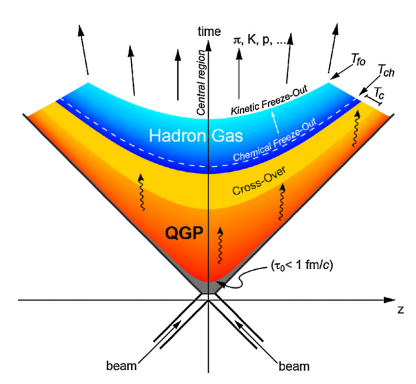
\includegraphics[width=0.6\linewidth]{images/collision_Phase.png}
		\caption{Space-time diagram of a heavy-ion collision of two nuclei colliding at time $t=0$ and longitudinal
position $z=0$ (transverse direction not shown). For details see text. Figure taken from ref.~\parencite{BRAUNMUNZINGER2019144}.}
		\label{fig:collision}
	\end{center}
\end{figure}

\begin{figure}
	\begin{center}
		\centering
		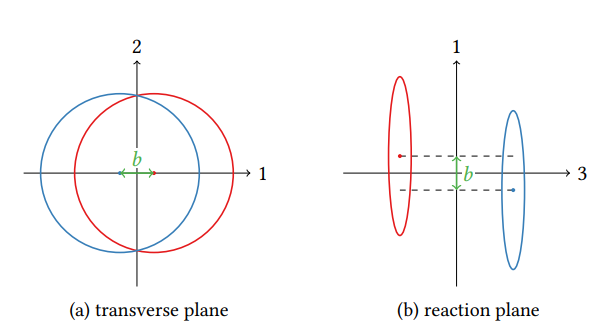
\includegraphics[width=0.8\linewidth]{images/collision_axes.png}
		\caption{Projection of the pre-collisional system onto the transverse plane (a) and reaction plane (b). Red and blue ellipses denote the forward- and backward-going
nuclei, respectively. The impact parameter is indicated by a green arrow.}
		\label{fig:collision_axes}
	\end{center}
\end{figure}

During a relativistic heavy-ion collision, two highly relativistic nuclei collide interpenetrating, giving rise to a complex cascade of interactions resulting in a shower of produced particles. Immediately after the initial contact, the nucleons of each ion are separated into two fragments: a group of "spectators", that continue to travel almost undisturbed along the beam axis, and a group of "participants", that interact with the opposing fragment. Due to the high density of particles, a hot fireball of
partonic matter forms between the receding fragments~\parencite{Bjorken1983}, where partons are deconfined, in a phase of matter called Quark-Gluon Plasma (\acrshort{qgp}). After a brief phase of strong dynamics, local thermal and chemical equilibrium is reached. The main characteristic of this phase, which can be described by relativistic fluid dynamics, is a rapid expansion both in the longitudinal and transverse directions and a consequent dilution and cool down of the fluid. Reached a critical temperature $T_\text{C}$~\parencite{Hagedorn1965}, the fluid hadronizes in a parton–hadron crossover. When the temperature and density drop even further, up to a point where interactions are too scarce to maintain kinetic equilibrium, particles “free stream” towards the detector, in a process described as kinetic freeze-out. A schematic space-time diagram of a heavy-ion collision in the longitudinal direction is depicted in fig.~\ref{fig:collision}. \\



Aspects of Heavy-ion collisions~\parencite{Wolschin2020}, hydro away from equilibrium~\parencite{romatschke2017} fast local thermalization sufficient for hydro~\parencite{Heinz2013}\\

In this thesis only symmetric collisions in which the two nuclei are identical in terms of their numbers of protons $Z$ and neutrons $A-Z$ are considered. In this scenario, the most convenient coordinate system to describe the collision is the \textit{center-of-momentum} (\acrshort{com})  frame, where the two ions move in the opposite direction with the same absolute momentum. The total energy available in the collision, if every nucleon would participate in the interaction, is the total relativistic energy in the \acrshort{com} frame $\sqrt{s}$. The maximum energy per nucleon pair $\sqrt{s_{\text{NN}}} = \sqrt{s}/A$ is also frequently used. The absolute relative longitudinal rapidity $y_\text{b}$ between the two rest frames of the incoming nuclei is usually called the \textit{beam rapidity}, and can be obtained from
\begin{equation}
\label{eq:beam_rap}
    y_{\mathrm{b}}=\operatorname{arcosh}\left(\frac{\sqrt{s_{\mathrm{NN}}}}{2 m_{\mathrm{N}}}\right), \quad m_{\mathrm{N}} \approx \frac{Z m_{\mathrm{p}}+(A-Z) m_{\mathrm{n}}}{A},
\end{equation}
where the average nucleon mass $m_\text{N}$ is approximated as a weighted average of the proton
mass $m_{\mathrm{p}} \approx 938.3$ MeV and neutron mass $m_{\mathrm{n}} \approx 939.6$ MeV, neglecting the binding energy of the nucleus. 

Just before the collision, the state of the system is determined by the wave function of the incoming nuclei. However, the latter is a complicated object, not yet fully understood, and we will thus approximate the nuclei with idealized perfect spheres in their respective rest frames, neglecting any substructure due to individual nucleons or partons. In the \acrshort{com} frame, these spheres are Lorentz-contracted to oblate spheroids, loosely referred to as "pancakes", moving parallel to the \textit{beam} or \textit{longitudinal axis}. The plane perpendicular to it is referred to as the \textit{transverse plane}, and projecting onto it the geometric centers of the nuclei yields two stationary points, whose distance is denoted as the \textit{impact parameter} $b$.

The origin of the cartesian coordinate is placed at the geometric center of the system, and the third direction is oriented along the beam axis. The first and second axes span the \textit{transverse plane}. Orienting then the first axis along the direction of $b$, it spans along with the longitudinal axis the \textit{reaction plane}. A schematic depiction of the system before the collision can be seen in fig.~\ref{fig:collision_axes}.\\

The focus of this thesis is limited to "central" collisions, in which the impact parameter $b$ does not exceed 5\% of the transverse size of the nuclei. Under this condition, the system possesses an approximate rotational symmetry around the longitudinal axis, that can be exploited by utilizing cylindrical coordinates $(p_\perp,\phi,p^3)$
\begin{equation}
    p_\perp := \sqrt{(p^1)^2+(p^2)^2}, \quad \quad \phi := \text{arg}(p^1 + ip^2),
\end{equation}
with $p_\perp$ being the \textit{transverse momentum}. Any physical observable expressed in the new set of coordinates, such as the stochastic trajectory of a particle, should then be in good approximation independent of the angle $\phi$. That implies that the stochastic process $\bm{P}$, after being expressed in cylindrical coordinates with the appropriate rules of stochastic calculus, can be reduced to a subprocess $(P_\perp,P^3)$ whose drift and diffusion coefficients are independent of the redundant stochastic variable $\Phi$.  


In addition, it is useful to transform the remaining momenta into hyperbolic rapidities. Firstly, $p^3$ is replaced by the \textit{longitudinal rapidity} $y$
\begin{subequations}
\begin{gather}
    y:=\text{artanh}\left(\frac{p^3}{p^0}\right), \\
    \frac{\partial\left(p_{\perp}, p^3\right)}{\partial\left(p_{\perp}, y\right)}=\left(\begin{array}{cc}
1  & 0 \\
\frac{\sinh (y)}{\sqrt{1+\left(m  / p_{\perp}\right)^2}}  & \sqrt{m ^2+p_{\perp}^2} \cosh (y)
\end{array}\right).
\end{gather}
\end{subequations}
This coordinate is particularly convenient for Lorentz transformations along the beam axis since the particle trajectory expressed in $\left(P_{\perp}, Y\right)$ can be boosted longitudinally by simply adding the relative boost rapidity $\Delta y$ to $Y(t)$ from the argument of the \acrshort{pdf},
\begin{equation}
f_{\left(P_{\perp}, Y\right)(t)+(0,\Delta y)}\left(p_{\perp},  y\right)=f_{\left(P_{\perp},Y\right)(t)}\left(p_{\perp}, y-\Delta y\right) .
\end{equation}
Lastly, $p_\perp$ is replaced by the \textit{transverse rapidity} $h$
\begin{subequations}
\begin{gather}
        h:=\operatorname{arsinh}\left(\frac{p_{\perp}}{m}\right), \\
        \frac{\partial\left(p_{\perp}, y\right)}{\partial(h, y)}=\left(\begin{array}{cc}
m  \cosh (h) & 0 \\
0  & 1
\end{array}\right),
\end{gather}
\end{subequations}
which maps low and high transverse momenta into a linear and logarithmic scale. 

\section{Drift-diffusion model}

As a final result of the collision, a shower of particles is measured by the surrounding detectors. After an accurate analysis of numerous events, the distribution of different particle species in phase space can be reconstructed. This information is encoded in the corresponding \textit{number density funcions} (\acrshort{ndf}s), denoted by $\mathrm{d}^nN/\mathrm{d}^n q$, where $\bm{q}$ is the relevant coordinate space, e.g. $(y,p_\perp)$. The total number of particles $N$ is obtained by integrating $\mathrm{d}^nN/\mathrm{d}^n q$ over the entire coordinate space. 
The connection to the \acrshort{pdf}s of a stochastic diffusion model is simply made by scaling the latter by the total particle number 
\begin{equation}
\label{eq:ndf_pdf}
   \frac{\mathrm{d}^nN}{\mathrm{d}^n q}(\bm{q}) = N f_{\bm{Q}}(\bm{q},t^*),
\end{equation}
where the stochastic process $\bm{Q}$ describes the trajectory of the particle of interest in $\bm{q}$-space that hit the detectors at some time $t^*$.

The coefficient functions for the \acrshort{fpe} of the process $\bm{Q}$ are obtained via the \acrshort{fdr} from an expected asymptotic state. However, eq.~\eqref{eq:fdr} only fixes the relation between the drift and diffusion coefficients, so another condition has to be set. Here, it will be assumed that the diffusion matrix for a process $\bm{\Xi} =(H,Y)$ in transverse and longitudinal rapidity, $\bm{\xi}=(h,y)$, is diagonal
\begin{equation}
    \bm{D}_{\bm{\Xi}} = \left(\begin{array}{cc}
D_\perp  & 0 \\
0  & D_\parallel
\end{array}\right).
\end{equation}
With this simplification, the drift coefficient can be completely determined from the asymptotic state with the \acrshort{fdr}~\eqref{eq:fdr_const_diff}.
This approach is in line with those used in the previous, one-dimensional iterations of the model. Although it is merely a lowest-order approximation, it will prove sufficient to obtain reasonable results. 

Under this anstatz, the \acrshort{fpe}~\eqref{eq:fpe} for the process $\bm{\Xi}$ assumes a particularly simple diagonal form


\begin{subequations}
\begin{equation}
  \frac{\partial}{\partial t} f_{\bm{\Xi}}(t)= \left[\operatorname{L}_{\bm{\Xi}}^{1}+\operatorname{L}_{\bm{\Xi}}^{2} \right]f_{\bm{\Xi}}(t),   
\end{equation}
with $\operatorname{L}_{\bm{\Xi}}^{i}$ containing only derivatives with respect to the coordinate $\xi^i$
\begin{gather}
\operatorname{L}_{\bm{\Xi}}^{1}(\bm{\xi})=D_{\perp} \frac{\partial}{\partial h}\left[-\frac{\partial \ln f_{\infty}(\bm{\xi})}{\partial h}+\frac{\partial}{\partial h}\right] \\
\operatorname{L}_{\bm{\Xi}}^{2}(\bm{\xi})=D_{\|} \frac{\partial}{\partial y}\left[-\frac{\partial \ln f_{\infty}(\bm{\xi})}{\partial y}+\frac{\partial}{\partial y}\right]
\end{gather}
\end{subequations}


\subsection{Dimentionless formulation}
Since rapidities are physically dimensionless, the only dimensionful quantities remaining in the associated \acrshort{fpe} are the time parameter $t$ and the diffusivity, having a dimension of time and inverse time, respectively. To eliminate these, the \acrshort{fpe} can be rewritten in terms of a new, dimensionless evolution parameter $\delta$ via $t=: t_0+\Delta t \delta$
\begin{equation}
    \frac{\partial}{\partial \delta} f_{\bm{\Xi}}(t_0+\Delta t \delta)=\Delta t \operatorname{L}_{\bm{\Xi}} f_{\bm{\Xi}}(t_0+\Delta t \delta), \quad \delta>0,
\end{equation}
with the interaction timespan $\Delta t:=t^*-t_0$. Here $t_0$ represents the initial time, and solving the equation up to $\delta=1$ corresponds to evolving it until the final time $t^*$.
Due to the shape of the \acrshort{fpo}, the diffusivity coefficients and interaction timespan can be combined to form the dimensionless products $D_{\perp} \Delta t$ and $D_{\|} \Delta t$, whose numerical values determine how close the final state is to the initial $\left(D_{\perp} \Delta t, D_{\|} \Delta t \ll 1\right)$ or asymptotic state $\left(D_{\perp} \Delta t, D_{\|} \Delta t \gg 1\right)$. This incidentally exposes an intrinsic symmetry of diffusive systems: changing the interaction timespan while reciprocally adjusting drift and diffusivity leaves the final state unchanged. Mathematically, this is related to a certain self-similarity of the standard Wiener process $W(t)$: for any constant $\alpha>0$, the process $\widetilde{W}(t):=\frac{1}{\sqrt{\alpha}} W(\alpha t)$ is also a standard Wiener process.
\\
%For the future, it is of course preferable to determine the diffusivity coefficient function from microscopic theories or phenomenological considerations; for example, by fixing the time evolution of macroscopic observables as discussed by Dunkel and Hänggi~\parencite{DUNKEL20091} for the case of binary elastic collisions in a heat bath. Specifically for the transverse direction, recent work by Caucal and Mehtar-Tani~\parencite{caucal2022} may be of interest in this regard.

\subsection{Multiple sources ansatz}
It is well known that in relativistic heavy-ion collisions energy and particle number densities are highly inhomogeneous in position space, so it can be expected that particle dynamics differ in space as well. This is not covered by the ansatz used in this thesis for the subprocess in momentum space $\bm{P}$, which assumes
that its coefficient functions do not depend on any positional coordinates. To address this issue at least partly, in previous applications of the model, the ansatz~\eqref{eq:ndf_pdf} was generalized by splitting the system into multiple disconnected subsystems (“sources”)~\parencite{Wolschin2006}
\begin{equation}
\label{eq:ndf_pdf_spurces}
   \frac{\mathrm{d}^nN}{\mathrm{d}^n q}(\bm{q}) = \sum_a N_a f_{\bm{Q}_a}(\bm{q},t^*), \quad \text{with} \quad \sum_a N_a = N,
\end{equation}
for which different initial and asymptotic states can be chosen, thereby decoupling their time evolutions with independent \acrshort{fpo}s $\operatorname{L}_{\bm{Q}_a}$. Conceptually, each source can be thought to occupy a distinct region in phase space, with overlap between the different regions deemed negligible. Although this approach has been proven successful, its implementation has revealed itself particularly challenging for the solution method based on the spectral eigenfunction decomposition of the \acrshort{fpo}. The reasons for that are discussed in a specific section of~\autoref{chap:particle_therm}, along with the nature and relative contribution of each source to particle thermalization at \acrshort{lhc} energies, and in the rest of this thesis only a single source is considered, with meaningful results obtained nonetheless. \\

References to include here or in the introduction: 


RDM with three sources~\parencite{Wolschin2015}
fragmentations sources in stopping~\parencite{Tani2009,Tani2009b}
non-equilibrium stopping~\parencite{Hoelck2020}

Particle production manustcript~\parencite{Hoelck2023}

\section{Spectral method of solution}

Spectral methods represent a powerful and versatile class of numerical techniques employed to solve partial differential and integral equations. Unlike traditional finite difference or finite element methods, the idea at the foundations of spectral methods is expressing solutions in terms of basis functions with global support. When applied to a smooth problem with a simple domain, spectral methods can achieve exceptional accuracy compared to other numerical methods, and the convergence is usually exponential in the number of basis functions or evaluation points. Among the abundant literature treating this broad subject, of particular help for the scope of this thesis was the textbook by~\textcite{Shizgal2015}, which covers in detail the application of spectral methods to kinetic theory and Fokker-Plank and Schrödinger problems, and the one by~\textcite{trefethen_spectral_2000}, that gives an introduction about their implementation in \textsc{Matlab}.

In this section, the use of non-classical orthogonal polynomials to efficiently construct a spectral representation of the \acrshort{fpo} will be discussed. Using such a basis set, it is possible to implement a representation of the one-dimensional operator that does not require an explicit calculation of the drift coefficient via the \acrshort{fdr}, while for the higher-dimensional case, the equivalence between the Fokker-Planck and a Schrödinger equation will be exploited. 


To construct a non-classical basis set, consider the polynomials $\{P_\text{n}\}$ orthonormal with respect to some weight function $w$ on $(\mathrm{a}, \mathrm{b}) \in \mathbb{R}$, that is,
\begin{equation}
    \label{eq:ort_pol}
    \int_a^b w(x) P_\text{n}(x) P_\text{m}(x) \mathrm{d} x=\delta_{\text{nm}} .
\end{equation}
The polynomials form a basis set and satisfy the general three-term recurrence relation~\parencite{davis2014}
\begin{equation}
    x P_\text{n}(x)=\sqrt{\beta_{\text{n}}} P_{\text{n}-1}(x)+\alpha_{\text{n}} P_\text{n}(x)+\sqrt{\beta_{\text{n}+1}} P_{\text{n}+1}(x),
\end{equation}
where the coefficients $\alpha_{\text{n}}$ and $\beta_{\text{n}}$ can be determined with the Stieltjes procedure developed by~\textcite{GAUTSCHI1985}. In this thesis, the \textsc{Matlab} adaptation \href{https://www.cs.purdue.edu/archives/2002/wxg/codes/OPQ.html}{\texttt{stieltjes.m}} of a \textsc{FORTRAN} routine~\parencite{GAUTSCHI1994} by the aforementioned author is used to generate the recurrence coefficients of an arbitrary weight function. 

\subsection{Spectral representation of the 1-$d$ FPO}

As seen in~\autoref{subsec:eig_exp} it is possible to bring the one-dimensional \acrshort{fpo} into a Hermitian form by multiplying it by $e^{\Phi}$, that is, by dividing it by the stationary solution $f_{X(\infty)}$\footnote{$f_{X(\infty)}$ is assumed to be normalized, such that all normalization factors are ignored in this section.}, but no explicit expression for this form was given. Writing the general time-dependent solution $f_{X}(x,t)$ as the product of the stationary solution and an auxiliary function $g_X(x,t)$
\begin{equation}
    f_{X}(x,t) := f_{X(\infty)}(x)g_{X}(x,t),
\end{equation}
the \acrshort{fpe} for the function $g_X$ becomes 
\begin{equation}
\label{eq:fpe_g}
    \begin{aligned}
\frac{\partial g_X}{\partial t} & =\frac{1}{f_{X(\infty)}} \frac{\partial}{\partial x}\left[D_X f_{X(\infty)} \frac{\partial g_X}{\partial x}\right]  \\
& =\mu_X \frac{\partial g_X}{\partial x}+D_X \frac{\partial^2 g_X}{\partial x^2}  =\operatorname{G}_Xg_X,
\end{aligned}
\end{equation}
where $G_X$ is self-adjoint with respect to the equilibrium solution as a weight function\footnote{With abuse of notation, in eq.~\eqref{eq:fpe_g} the same symbol as in eq.~\eqref{eq:fpo_herm} is used, even though in that case the self-adjointness of $\operatorname{G}_X$ was defined w.r.t. the unit function, and the two are thus different operators.}
\begin{equation}
\begin{aligned}
        \langle \phi_1 |\operatorname{G}_X | \phi_2 \rangle &= \int f_{X(\infty)}  \phi_1  \operatorname{G}_X  \phi_2 \mathrm{d}x \\
        &=\int f_{X(\infty)}  \phi_2  \operatorname{G}_X  \phi_1 \mathrm{d}x= \langle \phi_2 |\operatorname{G}_X | \phi_1 \rangle,  
\end{aligned}
\end{equation}
provided the zero flux boundaries condition
\begin{equation}
    \int_{\partial V} f_{X(\infty)}  D_X  \pdv{g}{x} \mathrm{d}x =0.
\end{equation}
To construct an efficient spectral representation of the operator $\operatorname{G}_X$, a basis of non-classical polynomials $\{P_\text{n}\}$ orthogonal w.r.t. the stationary solution of the \acrshort{fpe} can be employed. Such a basis satisfies eq.~\eqref{eq:ort_pol} with $w = f_{X(\infty)}$, and has the advantage that is automatically adapted to the specific problem. In addition, knowing that the first eigenfunction of the \acrshort{fpo} is the equilibrium distribution and that the successive eigenfunctions are orthogonal to it, a basis set satisfying the same orthogonality relations is intuitively "special" compared to other polynomial sets.
The spectral representation of $\operatorname{G}_X$ in this basis is~\parencite{shizgal1985,shizgal1996,Shizgal1998} 
\begin{equation}
\begin{aligned}
    \operatorname{G}_X^{\text{nm}} & =\int f_{X(\infty)} P_\text{n} \operatorname{G}_X P_\text{m} \mathrm{d} x \\
    & =\int f_{X(\infty)} P_\text{n} \frac{1}{f_{X(\infty)}} \frac{d}{d x}\left[f_{X(\infty)} D_X \frac{d P_\text{m}}{d x}\right] \mathrm{d}x
\end{aligned}
\end{equation}
Integrating by parts and making use of the orthogonality of the basis set w.r.t. the stationary solution, the expression simplifies to 
\begin{equation}
\label{eq:G_spec}
    \operatorname{G}_{X}^{\text{nm}}=\int f_{X(\infty)} D_X P_\text{n}^{\prime}P_\text{m}^{\prime}\mathrm{d}x,
\end{equation}
where natural boundary conditions were assumed. The representation~\eqref{eq:G_spec} is particularly convenient because it only requires polynomial derivatives that can be carried out analytically. Since the drift function does not explicitly appear in the expression, if one already knows the stationary solution and the form of the diffusion coefficient, as is the case in this thesis, the use of the \acrshort{fdr} is not even necessary. The eigenvalues $\lambda_\text{n}$ and eigenfunctions $\psi_\text{n}$ of the operator $\operatorname{G}_{X}$ can be estimated by diagonalization of the $N\times N$ symmetric matrix $\operatorname{G}_{X}^{\text{nm}}$, where $N$ is the dimension of the orthonormal basis set $\{P_\text{n}\}$. 
It was shown numerically that the coefficients of the expansion of $\psi_\text{n}$ in the $\{P_\text{n}\}$ basis set are linear variational parameters. The variational theorem then guarantees that this method provides an upper bound to the eigenvalues for each $N$ and converges from above.

The \acrshort{fpo} and $\operatorname{G}_{X}$ share the same eigenvalues, and are connected trough 
\begin{equation}
    \operatorname{G}_{X} = e^{\Phi} \operatorname{L}_{X} e^{-\Phi}.
\end{equation}
The time-dependent solution of the \acrshort{fpe} can be then approximated by 
\begin{equation}
\label{eq:fpe_exp_N}
    f_{X}(x,t) \approx  f_{X(\infty)}(x) \sum_{\text{n}=0}^{N-1} c_\text{n} \psi_\text{n}(x) e^{-\lambda_\text{n} (t-t_0)}, 
\end{equation}
where the coefficients $c_\text{n}$ are determined from the initial condition by
\begin{equation}
    c_\text{n} = \int f_{X}(x,t_0) \psi_\text{n}(x) \mathrm{d}x.
\end{equation}
The goodness of expression~\eqref{eq:fpe_exp_N} in approximating $f_{X(t)}$ depends of course on the convergence of the eigenvalues and eigenfunctions, but also on the convergence of the coefficients $c_\text{n}$ to zero approaching the $N-1$-th element. 


\subsection{Representation of the 2-$d$ Schrödinger operator}

~\parencite{shizgal1996}
equivalence to Susy~\parencite{Shizgal2016}

\chapter{Charged hadrons thermalization}\label{chap:particle_therm}

Due to the large number of particles present in the final stages of a relativistic heavy-ion
collision, it is to be expected that mutual interactions lead to an ongoing thermalization of
the system. However, the rapid expansion, particularly in the longitudinal direction, imposes limitations on the interaction time. This limitation arises both from the finite period until the hadrons reach the detectors and the dilution of the system due to its expansion, ultimately leading to a kinetic freeze-out. Consequently, it is expected~\parencite{Wolschin2006} that the system never attains thermal equilibrium but rather persists in a transient state at the time of measurement.

These circumstances provide favorable conditions for employing non-equilibrium statistical models, with a specific emphasis on drift-diffusion processes. The abundance of particles and interactions implies that correlations are likely to be negligible so that the impact of particle-hadron collisions can be effectively represented by a stochastic force acting on the hadrons. Concurrently, the collective expansion of the system and frictional interactions with the surroundings are expected to introduce an additional deterministic component to the motion of the hadrons, which a suitable drift coefficient can appropriately address.


Indeed, promising results could already be obtained by~\textcite{Wolschin1999,Wolschin2007} and~\textcite{Biyajima2002} with a simple one-dimensional Ornstein–Uhlenbeck ansatz, which was later refined through the use of a non-linear drift term based on a thermal \acrshort{fdr}~\parencite{Wolschin2019}. Here, the latest three-dimensional evolution of the diffusion model by~\textcite{Hoelck2023} is solved with a spectral eigenfunction decomposition, overcoming the numerical accuracy limitation of the latter that restricted the authors to obtain predictions beyond the low transverse momentum region ($p_\perp < 2$~GeV). 

\section{Initial state}

The thermalization process is modeled to begin directly after the production of particles from hadronic interactions of the colliding nuclei, and 
the system’s time evolution is set to start from this initial time $t_0$. The resulting trajectories are therefore to be interpreted in terms of \textit{parton–hadron duality} since many of the produced particles immediately dissolve into their partonic constituents, which only later reassemble into real hadrons. The associated initial \acrshort{pdf} are derived from a \acrshort{qcd}-inspired phenomenological framework based
on gluon saturation in the \textit{deep-inelastic scattering} (\acrshort{dis}) of participant partons~\parencite{GRIBOV1983,MUELLER1986,BLAIZOT1987,McLerran1994}, that was already successfully used by~\textcite{Hoelck2020} in the context of baryion stopping, and which appears to e compatible with a recent analysis of initial-state signals in ALICE data~\parencite{Acharya2022}. 

The key assumption of this framework is that the gluon density saturates below a characteristic momentum scale $Q_\text{S}$, so that the respective gluons form a \textit{color-glass condensate} (\acrshort{cgc}). For small values of the gluon’s Bjorken momentum fraction $x$, this scale can be parametrized as~\parencite{Golec1998}
\begin{equation}
    Q_\text{S}^2(x) = \sqrt[3]{A}Q_0^2 \left( \frac{x_0}{x}   \right)^\lambda,
\end{equation}
where the values $\lambda = 0.2$ and $\frac{4}{9}Q_0^2 x_0^\lambda = 0.09$ GeV$^2$ are used to be consistent with ref.~\parencite{Hoelck2020,Hoelck2023}. These values can be compared with literature results, where $\lambda \approx 0.288$ and $Q_0^2x_0^\lambda \approx 0.097$ GeV$^2$ were determined in a fit to deep-inelastic scattering e–p data from HERA~\parencite{Golec1998}.

The interaction of the participating nucleons is assumed to be mediated by quark-antiquark pairs (“dipoles”) emitted by the confined partons, which then inelastically scatter off the partons of the oppositely moving nucleus. Subsequent recombination of the involved quarks and gluons results in the production of new hadrons, which are emitted from the nuclear fragments. From the mass $m$ and rapidities $(h,y)$ of the produced hadron, the Bjorken momentum fractions $x_\pm$ of the two generating partons contained the forward $(+)$  and backward $(-)$ moving nucleon can be reconstructed from kinetic considerations
\begin{equation}
\label{eq:x_pm}
    x_\pm \approx \frac{m \cos(h) \exp(\pm y)}{2 m_\text{N} \sinh(y_\text{b})},
\end{equation}
with $y_\text{b}$ and $m_\text{N}$ as defined in eq.~\eqref{eq:beam_rap}. Note however, that equation~\eqref{eq:x_pm} is obtained by simply imposing energy and longitudinal momentum conservation, ignoring the initial transverse motion of the nucleons in the \acrshort{com} frame, as well as the comparatevely small parton masses contribution to the energy and any additional valence quarks that may be needed, and is therefore to be intended as an approximate estimation. \\


At low Bjorken $x$, the nucleon momentum is mostly carried by gluons, while valence quarks prevail at high $x$. For two interacting partons, this results in four dominant interaction processes for the \acrshort{dis} that constitute the disconnected sources present in eq.~\eqref{eq:ndf_pdf_spurces}: gluon-gluon (gg), gluon-valence quark (gq), valence quark-gluon (qg) and quark-quark (qq) interactions. As already anticipated, in this thesis, only one source is considered, the \textit{"central"} gluon-gluon scattering which predominantly yields hadronic particle-antiparticle pairs with low to intermediate $y$. Their initial \acrshort{pdf} can be approximated by~\parencite{KHARZEEV2005}
\sublabon{equation}
\begin{equation}
    \label{eq:pdf_initial_gg}
    f_{\bm{\Xi}(t_0)}(\bm{\xi}) \approx C_{\mathrm{gg}} \sinh (h) \cosh (h) \prod_{i \in\{+,-\}} x_i \frac{G\left(x_i ; m \sinh (h)\right)}{\sinh (h)^2} \Theta(1-x_i),
\end{equation}
where $G$ is the simplified gluon structure function
\begin{equation}
    x G(x ; Q) \propto(1-x)^4 \min \left(Q^2, Q_{\text{S}}^2(x)\right),
\end{equation}
\sublaboff{equation}
and $C_{\mathrm{gg}}$ is a numerically determined normalization constant. Eq.~\eqref{eq:pdf_initial_gg} is completely symmetric under the exchange of the forward- and backward-going gluon, and depends on the rapidity $y$ trough $x_\pm(y,h)$. The Heaviside theta functions are needed to ensure the validity of the Bjorken momentum fraction of the gluons since eq.~\eqref{eq:x_pm} has physical sense only for $x \leq 1$.

The hadron yield of the qq process is expected to be small in comparison with the other three and can thus be safely neglected, but one should not in principle ignore the contribution given by the interactions of gluons and valence quarks. These two "\textit{fragmentation}" sources produce particles at higher rapidities than the central source, and while essential to describe baryon stopping, their relevance in particle thermalization for central collisions at \acrshort{lhc} energies can be disregarded without heavy consequences. However, the reason why these sources are not included is simply the difficulty of accounting for their time evolution with the employed spectral eigenfunction decomposition, as illustrated in detail in~\autoref{sec:fragmentation}. 




\section{Asymptotic state}

Maxwell-Jüttner distribution~\parencite{Juttner1911}

\section{Fragmentation sources}\label{sec:fragmentation}



\section{Results}
Hagedron exponent estimate -8 ~\parencite{Phenix2011}~\parencite{aamodt_production_2011}~\parencite{MICHAEL19791}

\subsection{Convergence of the spectral decomposition}



\subsection{Parameter estimation and comparison with LHC spectra}
\begin{figure}
	\begin{center}
		\centering
		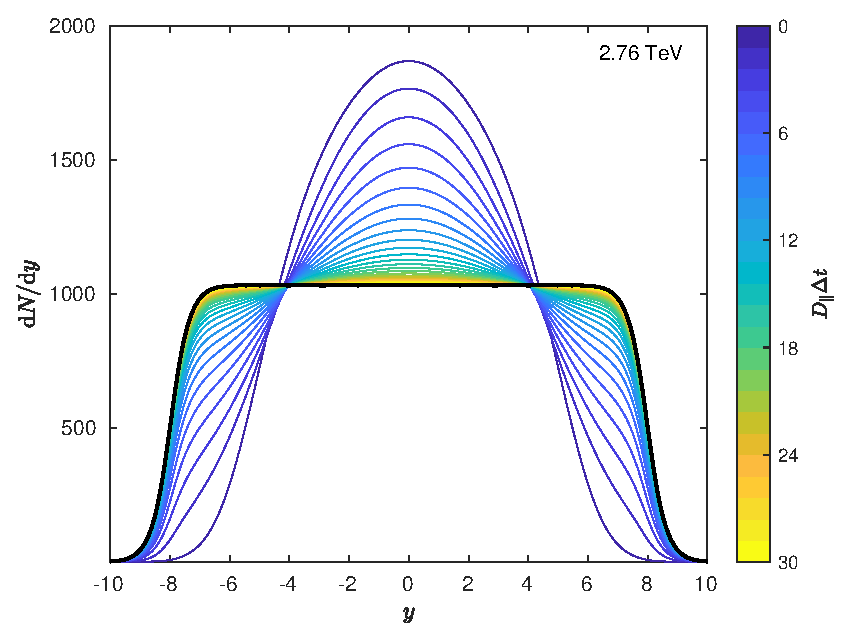
\includegraphics[width=\linewidth]{images/Pb_276_plot_y.eps}
		\caption{Time evolution of the marginal rapidity particle density function for Pb+Pb collision at 2.76 TeV}
		\label{fig:Pb_276_y}
	\end{center}
\end{figure}


\begin{figure}
	\begin{center}
		\centering
		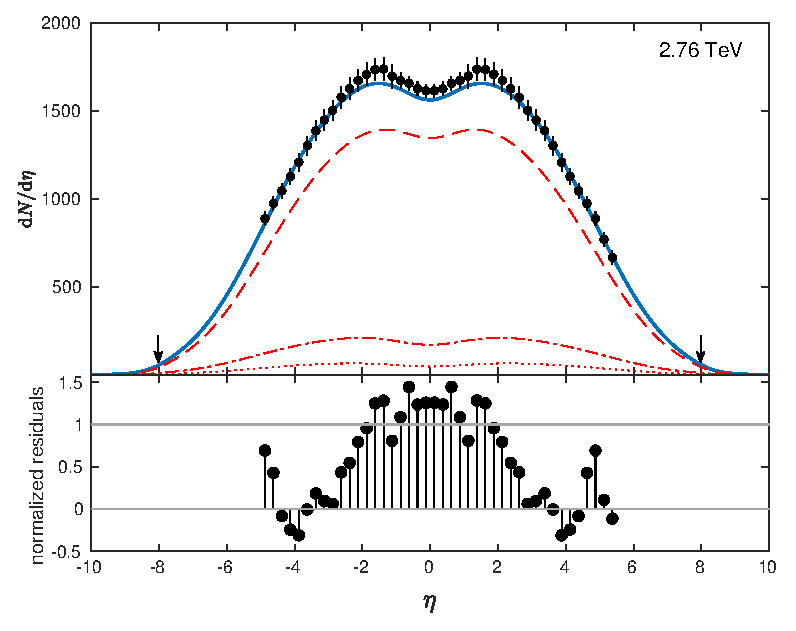
\includegraphics[width=\linewidth]{images/Pb_276_plot_eta.eps}
		\caption{Comparison with LHC data for Pb+Pb collision at 2.76 TeV for marginal pseudorapidity distribution}
		\label{fig:Pb_276_eta}
	\end{center}
\end{figure}


\begin{figure}
	\begin{center}
		\centering
		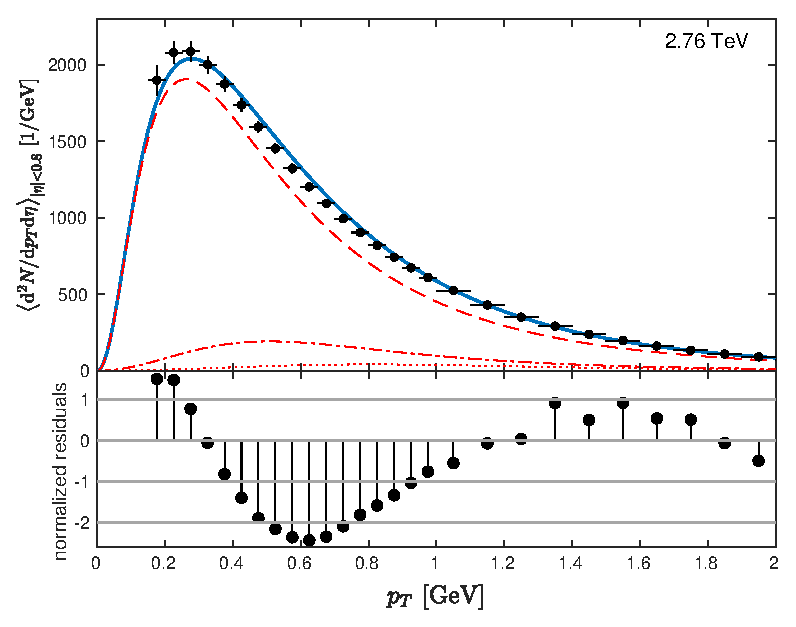
\includegraphics[width=\linewidth]{images/Pb_276_plot_pT.eps}
		\caption{Comparison with LHC data for Pb+Pb collision at 2.76 TeV for marginal transverse momentum distribution}
		\label{fig:Pb_276_pT}
	\end{center}
\end{figure}

\begin{figure}
	\begin{center}
		\centering
		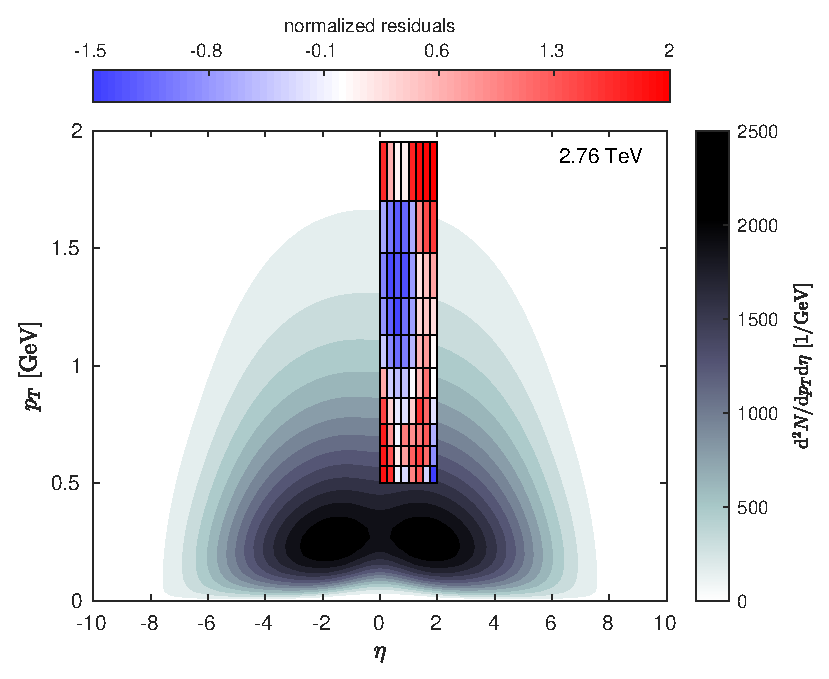
\includegraphics[width=\linewidth]{images/Pb_276_plot_2d.eps}
		\caption{Comparison with ATLAS data for Pb+Pb collision at 2.76 TeV.}
		\label{fig:Pb_276_2d}
	\end{center}
\end{figure}

\begin{figure}
	\begin{center}
		\centering
		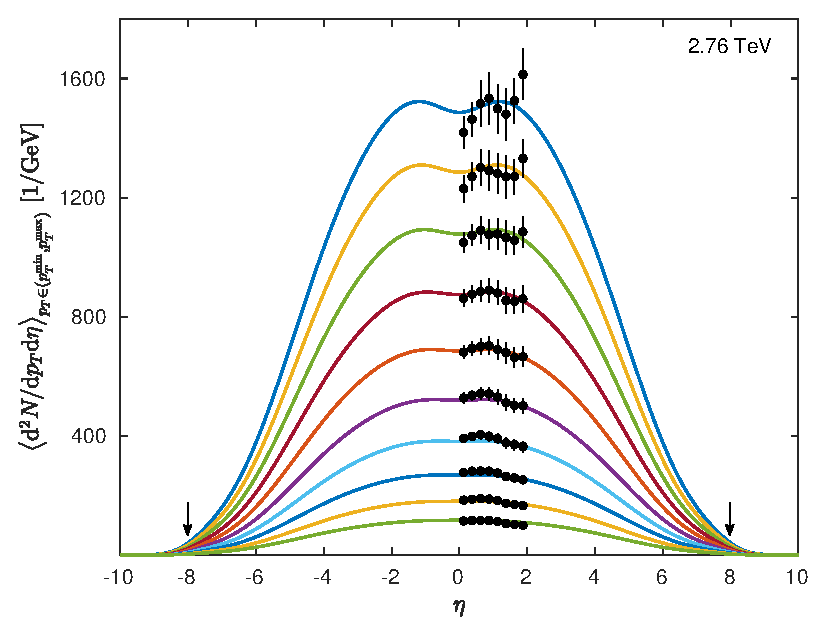
\includegraphics[width=\linewidth]{images/Pb_276_plot_2d_eta.eps}
		\caption{Comparison with ATLAS data for Pb+Pb collision at 2.76 TeV.}
		\label{fig:Pb_276_2d_eta}
	\end{center}
\end{figure}

\begin{figure}
	\begin{center}
		\centering
		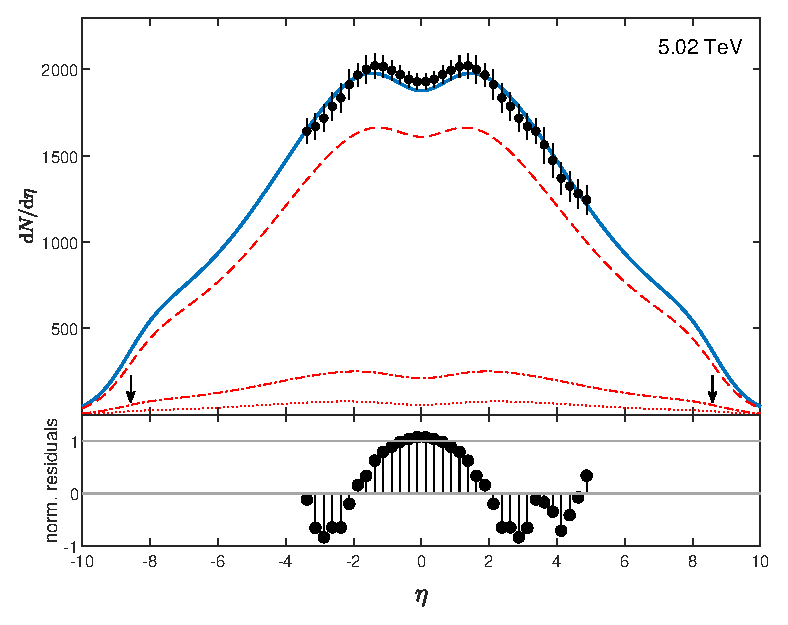
\includegraphics[width=\linewidth]{images/Pb_502_plot_eta_FP.eps}
		\caption{Comparison with LHC data for Pb+Pb collision at 5.02 TeV for marginal pseudorapidity distribution}
		\label{fig:Pb_502_eta}
	\end{center}
\end{figure}

\begin{figure}
	\begin{center}
		\centering
		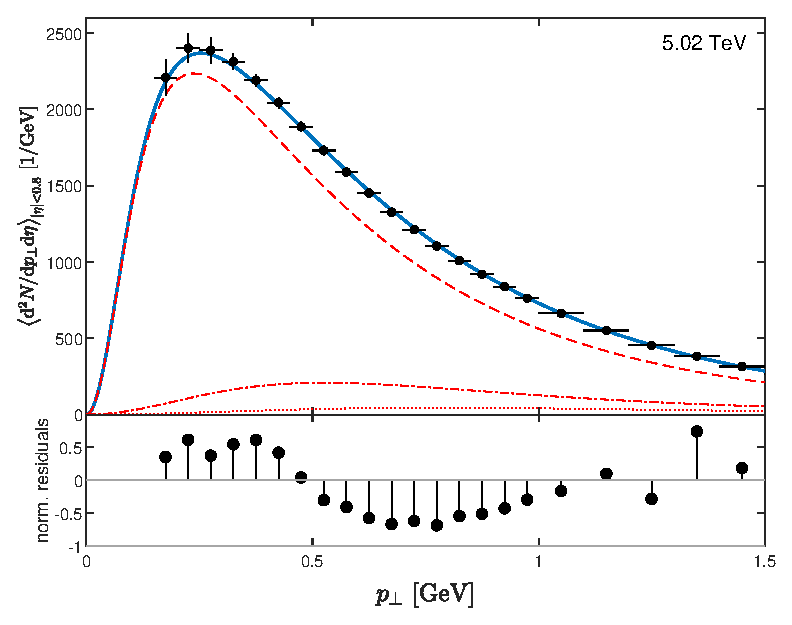
\includegraphics[width=\linewidth]{images/Pb_502_plot_pT_FP.eps}
		\caption{Comparison with LHC data for Pb+Pb collision at 5.02 TeV for marginal transverse momentum distribution}
		\label{fig:Pb_502_pT}
	\end{center}
\end{figure}

\begin{figure}
	\begin{center}
		\centering
		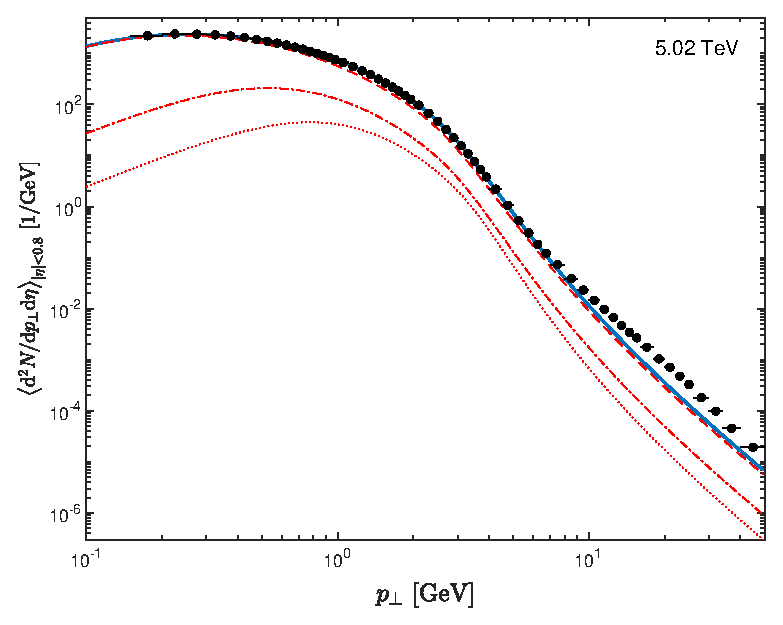
\includegraphics[width=\linewidth]{images/Pb_502_plot_pT_FP_loglog.eps}
		\caption{Comparison with LHC data for Pb+Pb collision at 5.02 TeV for marginal transverse momentum distribution}
		\label{fig:Pb_502_pT_loglog}
	\end{center}
\end{figure}

\subsection{Prevision for the current LHC run}
\begin{figure}
	\begin{center}
		\centering
		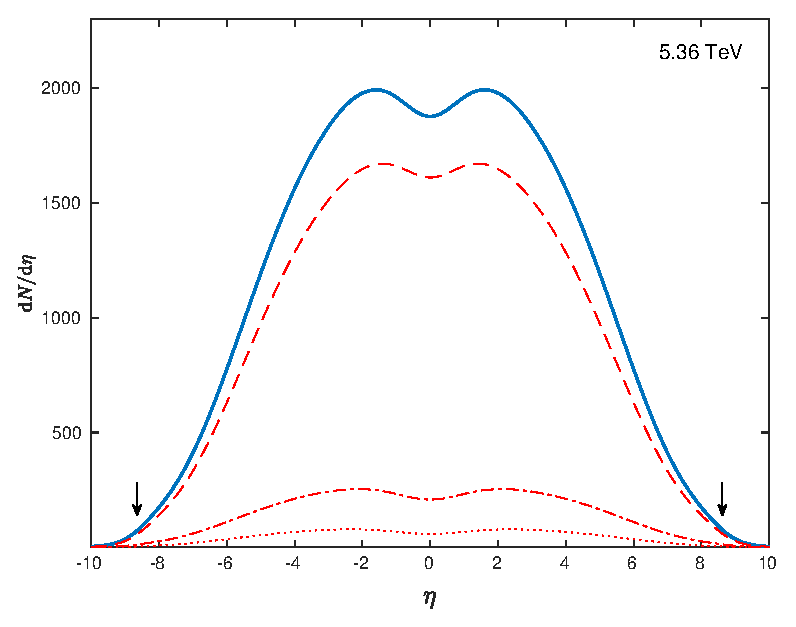
\includegraphics[width=\linewidth]{images/Pb_536_plot_eta.eps}
		\caption{Prevision of the pseudorapidity marginal distribution for Pb+Pb collision at 5.02 TeV.}
		\label{fig:Pb_536_eta}
	\end{center}
\end{figure}



\chapter{Conclusions}\label{chap:conclusions}


\printbibliography
\end{document}
